
\chapter{A Bayesian Random Partition Model for Sequential Refinement and Coagulation}
\label{ch:biometrics}
\index{Instructions for Preparing Dissertations, Theses, and Reports%
@\emph{Instructions for Preparing Dissertations, Theses, and Reports}}%

\section{Scientific publication}

This work has appeared in \cite{zanini2019}\footnote{Full citation: Zanini CTP, M\"uller P, Ji Y, Quintana FA (2019). A Bayesian random partition model for
sequential refinement and coagulation. \textit{Biometrics}.1-12. https://doi.org/10.1111/biom.13047}. Carlos Tadeu Pagani Zanini is the first author of the paper and worked on developing the overall inference approach, the MCMC algorithm for posterior estimation, designing the simulation study, analysing the data, identifying modifications to the model in response to observed lack of fit with the real data and also leading the drafting of the manuscript.

\section{Introduction}
\label{s:intro}

\subsection{Overview}

In this section, we propose a model for a sequence of partitions that includes refinement
of the initial partition followed by later coagulation. The model is
motivated by an analysis of protein activation over time after an
intervention.

A functional protein pathway involves proteins whose expressions are
dependent. For example, expression of a protein can stimulate the
expression of another protein. Usually a stable pathway leads to an
equilibrium state of the expression of all proteins in the pathway,
which can be modeled as a probability distribution. In cancer cells,
biological pathways are almost always disrupted, which shifts the
equilibrium state of the protein expression. Effective cancer drugs, such
as targeted protein inhibitors, can help treat cancer patients by altering protein expression for key biomarkers. Through pathways, other
proteins are subsequently affected which ultimately leads to phenotypes
that are beneficial for patient survival or quality of life. For a new
developmental drug, one of the first steps is to test which proteins are
affected when the drug is introduced to the cells. This is typically done
by functional assays. We consider such an assay in which protein
expression of a biological pathway is measured at the baseline and at
multiple time points after a drug is introduced to cancer cells.

We analyze protein expression data from such functional
assays. To investigate which proteins have their expression levels changed
(directly or indirectly) after being exposed to the drug, we define a
Bayesian model for protein expressions with a time-dependent clustering
structure. The underlying assumption of the model is a stylized
representation of the earlier description of disrupted protein pathways.
We assume that the proteins are originally clustered in a canonical way
with respect to their protein expressions and, after a certain time period
of drug exposure, some or all of the proteins have their expressions
altered, which may lead to a different clustering structure. As time
passes the drug effect wears off, and the clustering structure of the
proteins may revert to the initial state. In other words, we model
protein expression and the treatment 
effect by arranging proteins in different subsets (clusters), possibly
corresponding to biologic function, with cluster-specific mean
expression levels. Treatment response is modeled by allowing a change
in cluster-specific means over a time interval after treatment, and by
adding new clusters to allow for heterogeneous treatment responses.
The model includes random time points to define this time
interval after treatment. Methodologically, through a Bayesian modeling framework we propose
an approach that allows inference for such dependent and temporal
clustering. The dependence is on the partitions that define the
clusters, rather than on the distribution of these partitions.

The proposed process is a reduced and simplified version of the more
general fragmentation and coagulation process of \cite{TehAl:11}.
Another more general model, without explicit modeling of refinement or
coagulation,  is proposed in \cite{elliott2018} who use a hierarchical 
Dirichlet process to infer local genetic ancestry from genotype
data. The model implies a partition of subjects into subsets with common
ancestry at each locus. Partitions are allowed to vary across genetic
locus and dependence is formalized by a hidden Markov process.
In general, any
dependent discrete random probability model such as the Dirichlet 
or Pitman-Yor (PY) 
processes \citep{PIYO97}, indexed by discrete time, could be used to
induce the desired time-dependent random partition. Such models are
developed in \cite{caronetal:07} and \cite{rodriguez&terhorst:08}.
\cite{caronetal:07} construct a sequence of random partitions with each
partition marginally distributed as in a PY mixture model, with an
additional parameter to control similarity between partitions. The
approach is based on a property of the Ewens sampling formula known as
consistency under deletion \citep{kingman:78}. However, these models for
sequences of random partitions are more general than what is needed here
and the implied marginal distribution of the random partition at each time point is the same. In contrast, the assumed monotonicity of fragmentation and following
coagulation is important in our application. It represents how the
treatment affects the proteins (refinement), and that effect 
eventually vanishes  (coagulation). This desired monotonicity (of
adding and then removing clusters)
and the limited data in the motivating application 
lead us to construct a much simplified version of such more general
models. The main inference target is the subset of proteins that form the
refined partition clusters, corresponding to the desired subset of proteins
that are most affected by the initial treatment.

\subsection{Dataset}
\label{ss:dataset}

The motivating data are from an experiment using reverse phase protein
arrays (RPPA) which record the expression of selected proteins in a
biological pathway simultaneously on multiple samples. Multiple cell line
samples are prepared and exposed to multiple protein inhibitors
at different dose levels \citep{rppa_ref}.
The experimental design is a balanced factorial structure, including $C = 2$ cell
lines, $D = 3$ drugs, $J = 3$ technical replicates, and $L = 4$ doses (0,
0.625, 2.5 and 10uM), with expression measurements of $I=55$ proteins
recorded at $T = 8$ different times $(0, 5, 15, 30, 60, 90, 120$ and $180$
minutes) after the drug exposure.
The cell cultures are treated with three protein inhibitors that are often
investigated in cancer studies. The included drugs act on:
Phosphoinositide 3-Kinase (PI3K), which is responsible for coordinating
cell functions such as proliferation, cell survival, degranulation,
vesicular trafficking and cell migration \citep{pik3_ref}; Protein Kinase
B (AKT), which promotes growth factor-mediated cell survival, cell
proliferation and inhibits apoptosis through the inactivation of
pro-apoptotic proteins \citep{akt_ref}; and mitogen-activated protein
kinase kinase (MEK), which is an important component of the ERK1/2
signaling pathway that is often deregulated in cancer cells
\citep{mek_ref}.

Some of the data can be seen in the four panels in the left column of 
Figure \ref{fig:result_c1_d1}. The plots show the data for cell line
$c=1$ under drug $d=1$, which is the PI3K inhibitor. The horizontal
axis is time (in minutes) after treatment. The vertical axis is
protein expression (averaged over $J=3$ repeat experiments).
Notice how some proteins have their expressions altered after the dose
is administered.
Figure \ref{fig:result_c2_d1} shows the same for cell line $c=2$.

For an initial exploratory data analysis one could use a fit of the
trajectory for each protein and try to identify systematic changes. Figure \ref{fig:splines}, for example, shows a fit of the data using a
flexible regression model -- in this case smoothing splines. While the fit is reasonable, it remains difficult to spot proteins that respond to treatment.
By arranging proteins in clusters we will reduce some of the noise and
be able to highlight possible treatment effects.



\begin{figure}[tbp] 
\centering
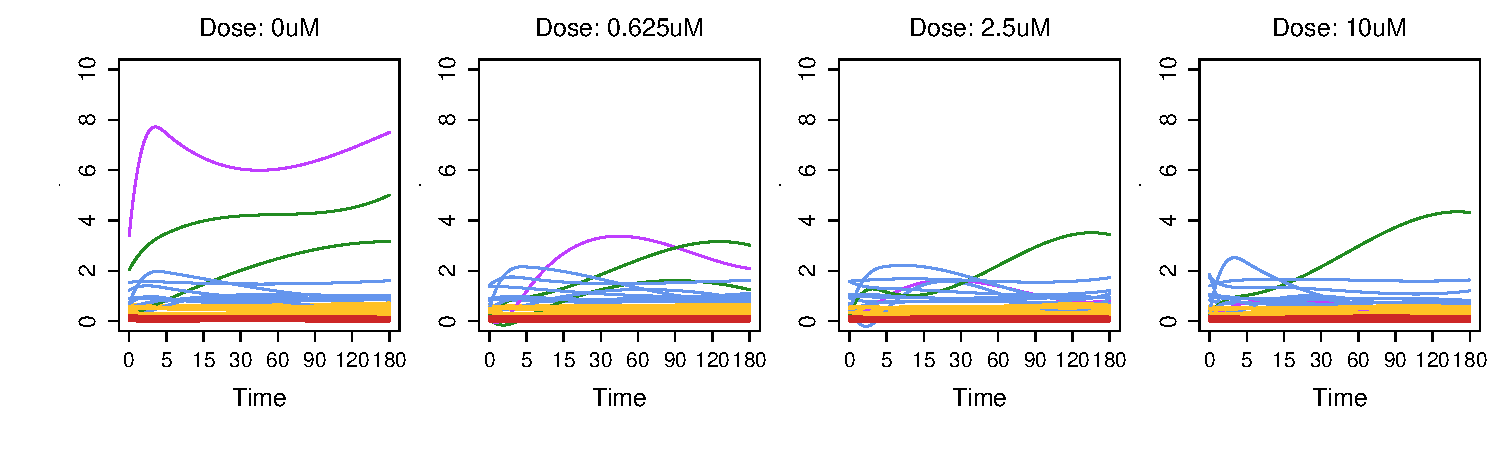
\includegraphics[scale=0.55]{figs_supporting_info/SuppInfo_ea_splines_11}
%\includegraphics[scale=0.6]{newfigs/ea_splines_11}
% \includegraphics[scale=0.6]{figs/fig5.jpeg}
\caption{Smoothing splines based on the J=3 repetitions over time (minutes) for each
protein in cell line 1 for drug PI3Ki. Cluster structure (represented in colors) is
constrained to be the same for all different doses.
Compare with the data shown in the left column of Figure 5.}
\label{fig:splines}
\end{figure}


\section{Probability Model}
\label{sec:model}

\vspace{0.5 cm}

Let $y_{cd\ell ijt}$ denote the expression level for protein $i$
in cell line $c$, drug $d$, dose $\ell$, replicate $j$ and time point $t$. To simplify notation, we drop $c$ and $d$ from the subindex in the following discussion as they appear in
(almost) all variables. Only one parameter, $\bfSigma_c$ is common across
drugs which we highlight by including the $c$ subindex for $\bfSigma_c$. In addition,
some of the hyperparameters are common across all $c,d$ as indicated below. 
We use notation for column vectors such as $(a_n)^N_{n=1} = (a_1, \ldots, a_N)^{\top}$.

We assume a model $y\lijt = \mu\lit + \epsilon\lijt,$ where $\mu\lit$ is the mean expression level for a specific cell line, drug, dose, protein and time, and $\epsilon\lijt$ represent time-dependent
Gaussian errors.
%
Let $\bfepsilon\lij = (\epsilon_{\ell ijt})^T_{t=1}$
denote the error vector. We assume $\bfepsilon_{\ell ij} \iid N(\bf0,
\bfSigma_c)$ with $\bfSigma_c$ denoting covariance matrix, independently across cell line, drugs, doses, proteins and
replicates. Similarly let $\bfy\lij = (y_{\ell ijt})^T_{t=1}$ and $\bfmu_{\ell i} = (\mu_{\ell it})^{T}_{t=1}$. The joint likelihood becomes
\begin{equation} \bfy\lij \ind N(\bfmu\li, \bfSigma_c),
  \label{eq:lik}
\end{equation} with independence across all subindex values, but dependence of the elements $y_{\ell ijt}$ across time $t=1,
\ldots, T$. We assume an inverse Wishart conjugate prior on the
covariance matrices $\bfSigma_c \ind \IW(\nu_{\Sigma}, \bfV_{\Sigma}),
\ c=1, \ldots, C,$ with expectation $\frac{\bfV_{\Sigma}}{\nu_{\Sigma}
- T - 1}$.
Here $\bfV_{\Sigma}$  is a (fixed) $T \times T$ matrix-variate hyperparameter
and $\nu_{\Sigma} \geq T + 2$ are the degrees of freedom. Introducing a more detailed model for temporal dynamics is
not meaningfully possible with the small sample sizes and only $T=8$
longitudinal observations. 

We introduce a time-dependent partition of the proteins, which
together with cluster-specific means implies a generative model for
the mean protein expressions $\bfmu\li$ within cell line, drug and
dose, and across different time points $t=1$, \ldots, $T$. We first
develop the structure for the time-dependent partitions.
Let $\bfdelta_t=(\delta_{ti})^I_{i=1}$
% \{S_{t}(1),\ldots, S_{t}(\kappa^t)\}$
denote the partition at time $t$
of proteins $i=1, \ldots, I$ into $\kappa^t$ clusters
$m=1,\ldots,\kappa^t$.
The random partitions $\bfdelta_t$ are characterized by cluster
membership indicators $\delta_{ti} \in \{1, \ldots, \kappa^t\}$ 
with $\delta_{ti} = m$ when protein $i$ is in the $m$-th cluster at time $t$.
A key model feature is the
prior probability model for the sequence of partitions
$\bfdelta_{1}, \ldots, \bfdelta_{T}$
that defines the evolution of the partitions over
time (as before, separately for each cell-line $c$ and drug $d$).
See below for the choice of $\kappa^t$ -- we will reduce it to only
two distinct values, $\kappa_1$ and $\kappa_2$, over time.
Also, for clarification we note that the dependence should be on the
partitions themselves rather than on their distributions.
Modeling the dependence on the actual proteins, i.e.,
the cluster membership of proteins, allows us to represent how the
treatment affects each protein.

One desired feature motivated by the nature of the RPPA data analysis
is that partitions should initially start fragmenting (i.e., more
subsets should be formed) up to a certain change point, after which a
coagulation process starts (i.e., merging of clusters into fewer
subsets). This reflects the drug action on proteins.  In other words,
the drug is expected to alter the regular expression pattern of the
proteins, resulting in more heterogeneous expression profiles and
therefore more clusters. As the drug effect wears off, the expression
of the proteins should revert to the original states, implying a
coagulation of the clusters.

We implement the desired structure with two change-points in time. The
first change point marks the beginning of the refined partition with more
clusters, and the second change point marks the time when the partition
reverts to the original clusters. We let $\tau^1_{\ell }$
(\textit{refinement} change point) denote the first change point when the
proteins form the finer partition, and let $\tau^2_{\ell }$
(\textit{coagulation} change point) denote the second change point.
We assume $1 \leq \tau^1_{\ell}
< \tau^2_{\ell } \leq T$ for all cell lines $c$, drugs $d$, and doses
$\ell$. One key feature is that $\tau^1_{\ell }$ and $\tau^2_{\ell}$ are
specific to dose $\ell$. This represents how different doses act
faster or slower on the proteins. Higher doses are expected to start
acting on the proteins earlier than lower doses, i.e., we expect
monotonicity of $\tau^1_{\ell}$ and $\tau^2_{\ell}$ over doses. We further
assume $
  (\tau^1_{\ell }, \tau^2_{\ell}) \iid \Unif\left(\{ (u_1, u_2): 1
\leq u_1 < u_2 \leq T-1\}\right).
$ Adding an informative prior would be straightforward. However, even
with the (vague) uniform prior we find little posterior uncertainty
on the change points.

The prior probability models for the baseline and fragmented partitions
are constructed as Dirichlet-multinomial models for cluster membership
indicators. Let $\bfdelta^u =(\delta^u_i)^I_{i=1}$ for $u\in \{1, 2\}$ denote the two partitions of
proteins with $u=1$ indicating the original (coarse) partition that applies for $t <
\tau^1_{\ell}$ and $t>\tau^2_{\ell}$, and $u=2$ indicating the (refined) partition
that applies for $\tau^1_{\ell} \leq t \leq \tau^2_{\ell}$. That is,
\begin{equation*}
\bfdelta_{t}=
\begin{cases}
  \bfdelta^1, \mbox{ for }
  1\leq t \leq \tau^1_{\ell }, \mbox{ or } t \geq \tau^2_{\ell }+1 \\
  \bfdelta^2, \mbox{ for } \tau^1_{\ell }+1 \leq t \leq \tau^2_{\ell }.
\end{cases}
\end{equation*}

We assume that 
$
P(\delta^1_i = m) = \pi^1_m
% (1), \ldots, \delta^1(I) \iid
%    \Cat(\{1,\ldots,\kappa_1\}, (\pi^1_1, \ldots, \pi^1_{\kappa_1}) ).
$
for clusters $m=1, \ldots, \kappa_1$.
The prior for the fragmented partition $\bfdelta^2$ is constructed in two steps. First, set
$\delta^2_i = \delta^1_i$ with probability $\gamma$; second, all
proteins $i$ with $\delta^2_i \not=\delta^1_i$ are gathered in the set
$\AAA:=\{i: \ \delta^1_i \neq \delta^2_i\}$, and form new
clusters by $P(\delta^2_i=m) = \pi^2_{m-\kappa_1},~ m=\kappa_1+1,\ldots,\kappa_2, \ i \in \AAA.$ Note that $p(\bfdelta^2 \mid \bfdelta^1)$ does not define $\bfdelta^2$
as a partition nested within $\bfdelta^1$.  This is why we use
the term refinement throughout. 

We assume independent priors for $\gamma$,
  $\bfpi_1=(\pi^1_1,\ldots,\pi^1_{\kappa_1})$ and
  $\bfpi_2=(\pi^2_1,\ldots,\pi^2_{\kappa_2-\kappa_1})$ as
$
   \gamma \sim \mbox{Beta}(a_\gamma, b_{\gamma})\
   \bfpi_1 \sim \Dir(\bfeta_1), \mbox{ and } \
   \bfpi_2 \sim \Dir(\bfeta_2).
$
The hyperparameters $\gamma, \bfpi_1, \bfpi_2$ are shared across all cell
lines $c$ and drugs $d$. 

Next, we construct a prior for the mean protein expression
$\bfmu\li$ in \eqref{eq:lik} by defining cluster-specific common
values.
% \bch $(\mu^*_{\ell,1}(m),\mu^*_{\ell,1}(m),\mu^*_{\ell,3}(m))$ for
% proteins in cluster $m$, under dose $\ell$ over interval $u=1,2,3$. \ech
That is, the partition is linked with the protein mean expression.
Given  $\{\bfdelta_{t}: \ 1\leq t \leq T\}$ we assume
\begin{equation}
\mu\lit=
\begin{cases}
\mu^*_{\ell 1}(\delta^1_i), \mbox{ if } 1\leq t \leq \tau^1_{\ell }\\
\mu^*_{\ell 2}(\delta^2_i), \mbox{ if } \tau^1_{\ell }+1 \leq t \leq \tau^2_{\ell }\\
\mu^*_{\ell 3}(\delta^1_i), \mbox{ if } \tau^2_{\ell }+1 \leq t.
\end{cases}
\label{eq:mu_vec}
\end{equation}
In words, $\mu\lit = \mu^*_{\ell u}(m)$ for all proteins in cluster $m$ under
dose level $\ell$ in the time interval $u=1,2$ or $3$, with the time
intervals corresponding to the initial, fragmented and final partitions respectively (initial and final partitions are assumed equal). The choice of the piecewise constant mean function in
\eqref{eq:mu_vec} is only for parsimony. Alternatively, one could use
a piecewise linear mean response, without much change in the remaining
discussion. The use of a distinct $\mu^*_{\ell 3}$, i.e. $\mu^{*}_{\ell 3}=\mu^{*}_{\ell 1}$ allows for a persisting effect of the drug intervention, short of a complete restriction to baseline.

The model is completed with a prior on the cluster-specific parameters, $  (\mu^*_{\ell u}(m)\mid \mu_{0u}, v_{0u}) \iid N(\mu_{0u}, v^{-1}_{0u}), \
  \mu_{0u} \iid  N(\mu_{00}, v^{-1}_{00}) \ \mbox{and} \
  v_{0u}   \iid  \mbox{Gamma}(a_v, b_v).$
The hyperparameters $(\mu_{0u},v_{0u})$ are common across cell lines $c$
and drugs $d$. 

In summary, the proposed model constructs a mixture of Gaussian sampling model
for the observed protein expressions over time, with the mixture being
induced by the latent partitions $\bfdelta^1$ and $\bfdelta^2$.
In fact,  marginalizing $\bfdelta^1$ and $\bfdelta^2$, we find the
following mixture of normals sampling model.
Let
$\bfu_1 = (1, \ldots, 1, 0, \ldots, 0)^{\top}$,
$\bfu_2 = (0, \ldots, 0, 1, \ldots, 1, 0, \ldots, 0)^{\top}$ and
$\bfu_3 = (0, \ldots, 0, 1, \ldots, 1)^{\top}$
denote design vectors with 1's in positions $1,\ldots,\tau^1_{\ell}$
(for $\bfu_1$), 
in positions $\tau^1_{\ell}+1, \ldots, \tau^2_{\ell}$ (for $\bfu_2$) and
in positions $\tau^2_{\ell} + 1, \ldots, T$ (for $\bfu_3$), respectively, and
let
$
\bfmu^*_{\ell}(k_1, k_2) = \mu^*_{\ell 1}\left(k_1\right)\bfu_1 +
\mu^*_{\ell 2}\left(k_2\right)\bfu_2 + \mu^*_{\ell
  3}\left(k_1\right)\bfu_3
$
denote the $T$-dimensional mean vector for proteins in clusters $k_1$
and $k_2$ under the initial and the refined partition, respectively. Let $N(\bfx;\, \bfm, \bfS)$ denote a multivariate normal p.d.f. evaluated at $\bfx$ with mean $\bfm$ and covariance matrix $\bfS$. Then
\begin{multline*}
p(\bfy_{\ell ij} \mid \tau^1_{\ell}, \tau^2_{\ell}, \bfSigma_c, 
 \bfmu^*_{\ell 1}, \bfmu^*_{\ell 2}, \bfmu^*_{\ell 3}, \bfpi_1,
 \bfpi_2, \gamma)=\\
= (1-\gamma) \sum^{\kappa_1}_{k_1=1}\sum^{\kappa_2-\kappa_1}_{k_2=1} 
   \pi^1_{k_1}\pi^2_{k_2}N(\bfy_{\ell ij} ; \bfmu^*_{\ell}(k_1, k_2), \bfSigma_c) \
+ \\ 
+\gamma \sum^{\kappa_1}_{k_1 = 1} 
   \pi^1_{k_1}N(\bfy_{\ell ij} ; \bfmu^*_{\ell}(k_1, k_1),
   \bfSigma_c). 
 \label{eq:marginal_likelihood} 
\end{multline*}

Note how the proposed model is different from models that allow dependence
of the distributions for the random partitions. 
Dependence in the prior on the random partitions over time would not necessarily
enforce the desired monotonicity of refinement (to represent the
treatment effect) and following coagulation for an actual realization
of protein-specific cluster membership.
Here, the dependence is built on the partitions themselves, unlike,
for example, the earlier 
mentioned model of \cite{caronetal:07} where each $\bfdelta_t$ is marginally
distributed according to a PY-style (Generalized P\'olya urn) distribution, 
exploring several ways to relate and control similarity across partitions.
The fragmentation
and coagulation feature cannot be represented by models with invariant
marginal distribution. Modeling the desired monotone pattern of change in
the partition is the key motivation for the proposed construction.

Finally, we would like to comment on the choice of the proposed model
versus a seemingly simpler parametric model, such as a linear mixed
effects model or a regression with splines, as in Figure 1 in the supporting information section.
While such parametric models could adequately model time-dependent
mean response, inference for protein-specific response to treatment
effects would require corresponding protein- and time-specific random
effects.

\section{Posterior Inference}
\label{sec:inference}

We implement Markov chain Monte Carlo (MCMC) posterior simulation.
Let $\bftheta$ denote the complete
parameter vector. For posterior simulation it is now important to keep
track of parameters that are in common across cell lines $c$ and drugs
$d$. We therefore start to include the subindexes $c$ and $d$ again as needed.
The joint prior distribution can be factorized as
\begin{align*}
p&(\bftheta) \propto
 \left\{\prod^3_{u=1}p(v_{0u})\right\}
 \left\{\prod^3_{u=1}p(\mu_{0u})\right\}
 \left\{\prod^C_{c=1}\prod^{D}_{d=1}\prod^L_{\ell=1} p(\tau^1_{cd\ell}, \tau^2_{cd\ell})\right\}
 p(\gamma)\\
%
&\times \left\{\prod^C_{c=1}\prod^D_{d=1}
  p(\bfdelta_{cd}^1\mid \bfpi_1)
  p(\bfdelta^2_{cd} \mid \bfdelta^1_{cd}, \gamma, \bfpi_2)\right\} \times
  p(\bfpi_1) p(\bfpi_2) \times
 \prod^{D}_{d=1} \prod^{C}_{c=1}p(\bfSigma_c)\\
%
& \times  \prod^C_{c=1} \prod^D_{d=1} \prod^L_{\ell=1}
  \left\{
  \underbrace{
  \prod^{\kappa_{1}}_{m=1}p(\mu^*_{cd\ell 1}(m) \mid \mu_{01}, v_{01})
  }_{u=1}\times
  \underbrace{
    \prod^{\kappa_{2}}_{m=1}p(\mu^*_{cd\ell 2}(m) \mid \mu_{02}, v_{02})
  }_{u=2} \times\right.\\
%
&\times \left.
  \underbrace{
    \prod^{\kappa_{1}}_{m=1}p(\mu^*_{cd\ell 3}(m) \mid \mu_{03}, v_{03})
  }_{u=3}
\right\},
\end{align*}
where $\kappa_{1}$ is the number of
clusters in time intervals $\{t: \ 1\leq t \leq \tau^1_{cd\ell}\}$ (corresponding
to $u=1$) and $\{t: \ t > \tau^2_{cd\ell}\}$ (or $u=3$); and $\kappa_2$ is the number of clusters in time interval $\{t: \ \tau^1_{cd\ell}+1\leq t \leq \tau^2_{cd\ell}\}$ (or $u=2$). 
If desired, the model could easily be generalized to different number of clusters
across cell line and drugs. The likelihood is given by the independent normal sampling model
$$
 \prod^{C}_{c=1} \prod^{D}_{d=1} \prod^{I}_{i=1} \prod^{L}_{\ell=1}
 \prod^{J}_{j=1} N( \bfy_{cd\ell ij}; \ \bfmu_{cd \ell i}, \  \bfSigma_c).
$$
Although posterior inference is not analytically tractable for this model,
conditional conjugacy implies that all full conditionals are well known
distributions that are straightforward to sample from (see Web Appendix
A). We therefore implement MCMC simulation using a Gibbs
sampler Markov chain.
We run one common Markov chain for inference across all $(c,d)$,
but report inference on partitions separately for each $(c,d)$. Therefore, in the
following discussion of inference summaries, we drop the
$_{cd}$ subindex again. 

Point estimates of the cluster-membership indicators are obtained using the
approach proposed by \cite{dahl2006}. After
judging (practical) convergence of the MCMC algorithm, we evaluate for each pair $i<j$ of
proteins, the pairwise co-clustering probability $\phat_{ij} = \frac 1K
{\sum_k} \pijk$, where $K$ is the Monte Carlo sample size and $\pijk$ is
an indicator for $i$ and $j$ being allocated to the same cluster. The
$\pijk$ and $\phat_{ij}$ are combined into $(I \times I)$ matrices
$\bfPk = [\pijk]$ and $\bfPhat = [\phat_{ij}]$. We then report as
posterior estimated $\bar{\bfdelta}$ the partition corresponding to the $\bfP^{(k^*)}$
% co-clustering matrix $\bfPs$
% cluster in iteration $k$, and 0 otherwise. Finally, the cluster
% membership indicator are punctually estimated by the $\bfP^{(k^*)}$
that minimizes $ ||\bfPhat - \bfP^{(k)} ||$, i.e.,
$
  k^\star = \arg\min_k || \hat{\bfP} - \bfP^{(k)} ||.
$
% Notice that such procedure takes the entire posterior sample into
% consideration and, since only one of those iterations is used to get
% the final point estimate for the clusters, problems with label
% switching are avoided.
In words, $k^\star$ indexes the Monte Carlo sample whose co-clustering
matrix is closest to $\bfPhat$. Once the point estimate of the
clustering structures is obtained, we run a new MCMC chain with fixed
cluster membership indicators to carry out inference for the remaining
parameters, now conditional on the estimated partition.

Finally, we consider learning about the unknown size $\kappa_1$ and
$\kappa_2$ of the partitions.
Using transdimensional transition probabilities, such as reversible jump
\citep{green1995},
the selection of these parameters could be included
in the same MCMC simulation.
However, we found that the implementation of such transition
probabilities is impractical for the proposed model. Considering a
variation of reversible jump for multivariate mixtures of normals with split and
merge proposals that are constructed to maintain marginal first and
second moments
\citep{zhang2004,Dellaportas2006}
we find it impossible to achieve acceptable mixing rates of the Markov
chain simulation. The challenge lies in finding a split move that simultaneously proposes reasonable draws for $\mu^*_{cd\ell u}(m)$ across all $\ell\in \{1, \ldots, L\}$, $u\in \{1, 2, 3\}$ and $m\in \{1, \ldots, \kappa_1\}$ with high probability. We therefore recommend to use an alternative model
selection framework to determine $(\kappa_1,\kappa_2)$.
We consider several criteria, including AIC \citep{akaike1973}, BIC
\citep{schwarz1978}, DIC \citep{spiegelhalter2002}, and WAIC
\citep{watanabe2010} as well as log pseudo marginal likelihood (LPML).
See, for example, \cite{gelman2014} for a review on these methods. The
specifics of counting the number of parameters, as it is required to
evaluate AIC and BIC are described in Web Appendix B.
In the following section we report a specific recommendation, based on
results in a simulation study. 

\section{Simulation}
\label{sec:simulation}

We carried out several simulation studies to verify that the proposed
model allows for meaningful inference in the context of weak signals
and relatively small sample sizes as in the RPPA data.  We considered
two scenarios, with several variations.
\smallskip

\underline{Scenario 1:}
We simulated five hypothetical datasets with the following
(true) partition sizes: $(\kappa_1, \kappa_2) \in \{ (2,3), (3,4), (3, 5), (4,7),
(5,7)\}$. In all five cases we simulated from the model described in
section \ref{sec:model}. The bottom level hyperparameters were fixed as
$\gamma = 0.9$, $v_{0u} = 5$ for $u = 1, 2, 3$ and $\bfSigma_c = 0.1 I_{8\times 8}$, where $I_{8\times 8}$ denotes the 8 dimensional identity matrix.
For any cell line $c$ and dose $\ell$, the change points were fixed as
$(\tau^1_{cd\ell}, \tau^2_{cd\ell}) = (2, 5)$ for $d = 1$, $(\tau^1_{cd\ell}, \tau^2_{cd\ell}) = (3, 6)$
for $d=2$ and $(\tau^1_{cd\ell}, \tau^2_{cd\ell}) = (4,7)$ for $d=3$. For
$(\kappa_1, \kappa_2) = (2,3), (3,4), (3, 5),$ we fixed $\mu_{0u} = (0.5,
1.5, 0.4),$ whereas for $(\kappa_1, \kappa_2) = (4,7), (5,7),$ we fixed
$\mu_{0u} = (1.0, 1.5, 1.4).$ The remaining parameters were randomly
generated from the respective prior probability model. 

For each dataset we then implement inference in two steps as in section
\ref{sec:inference}. First we run 500 MCMC iterations,
discarding the first 100 as initial burn-in
under each one of 21 possible pairs of $(\kappa_1,\kappa_2)$. We use the pairs
$\{(a,b): a \in \{2,\ldots, 8\}, \ b \in \{a+1, a+2, a+3\} \ \}$.
This first step evaluates the different model choice
criteria (see below) to select the best pair $(\kappa_1, \kappa_2)$,
and then estimates $(\bfdelta^1_{cd},\bfdelta^2_{cd})$ using the approach of
\cite{dahl2006}.

In a second step we simulate 5000 more MCMC iterations
to implement inference conditional on the
chosen model, i.e., with fixed
$\bfdelta^1_{cd}, \ \bfdelta^2_{cd},$ \  $c=1,2, \ d = 1,2,3$.
The first 2000 iterations are discarded as initial burn-in.
Hyperparameters are fixed
as $\nu_{\Sigma} = 10$, $\bfV_{\Sigma}=I_{8\times 8}$,
$a_{\gamma}= 1$, $b_{\gamma}= 1$, $\bfeta_1= (1,...,1)^{\top} \in
\mathbb{R}^{\kappa_1}$, $\bfeta_2=(1,...,1)^{\top} \in
\mathbb{R}^{\kappa_2 - \kappa_1}$, $\mu_{00}=0$, $v^{-1}_{00}=0.4444$,
$a_v=1$ and $b_v=1$ to reflect weak prior information.

We implement learning about the cluster sizes
$(\kappa_1,\kappa_2)$ as model selection using various criteria
proposed in the literature. We briefly summarize the results in Table
\ref{tab:IC}. BIC always selects a more parsimonious model, and AIC, DIC,
WAIC and LPML always point to the same model (except under $(5,7)$). We
conclude to use BIC, as it gives the best trade-off of a good fit and
selecting parsimonious models.


\begin{table}[tbp]
\caption{Simulation truth and estimate for $(\kappa_1,\kappa_2)$ under
  alternative model selection criteria.
  $^\star$ Under simulation truth $(5,7)$, AIC selects $(5,6)$.
}
\centerline{
  \begin{tabular}{l|ccccc} % |
%% no clue what's going on -- my emacs needs a second "|" lest it
%% messes up color coding of the latex source :-)
    truth & (2,3) & (3,4) & (3,5) & (4,7) & (5,7)\\
    \hline
    BIC   & (2,5) & (2,5) & (3,4) & (3,6) & (5,6)\\
    AIC, DIC,WAIC, LPML & (4,7) & (3,6) & (5,6) & (4,7) & (8,10)$^\star$
  \end{tabular}
}
\label{tab:IC}
\end{table}



Next we summarize results for the simulation scenario with true $(\kappa_1, \kappa_2) \\ = (3,
5)$. In this case BIC selects $(\kappa_1, \kappa_2) = (3, 4)$. The objective is to explore whether inference can
recover mean parameters and cluster structure for data with sample
sizes and complexity comparable to the motivating RPPA study.
%  demonstrate that the inference
% procedure is capable of reasonably estimating the mean parameters and
% cluster structure under the hypothesis that data comes from the model,
% with the same sample size as the dataset analyzed in section
% \ref{sec:results}.
Figure \ref{fig:simulation_cluster_membership} shows
estimated partitions under coagulation and refinement,
arranged by cell line and drug
$(c,d)$. In a few cases, we get estimates that merge two (true)
clusters together (e.g., in the estimated partitions $\bfdelta^1_{cd}$
and $\bfdelta^2_{cd}$ for $(c,d)=(1,3)$ and for $(c,d) = (2,1)$).
% $\delta^1_{13}, \delta^1_{2,1}$).
In most cases, however, the underlying cluster structure is accurately
recovered and we are able to correctly identify which proteins
are affected by the respective drug (proteins corresponding to darkest shades of gray in plot (b)).

\begin{figure}[tbp]
  \begin{center}
  \begin{tabular}{cc}
     Cell line 1 \hspace{0.5 cm} Cell line 2 & 
     Cell line 1 \hspace{0.5 cm} Cell line 2\\
    \rotatebox{90}{drug 1 \hspace{0.1cm} drug 2 \hspace{0.1cm} drug 3}
    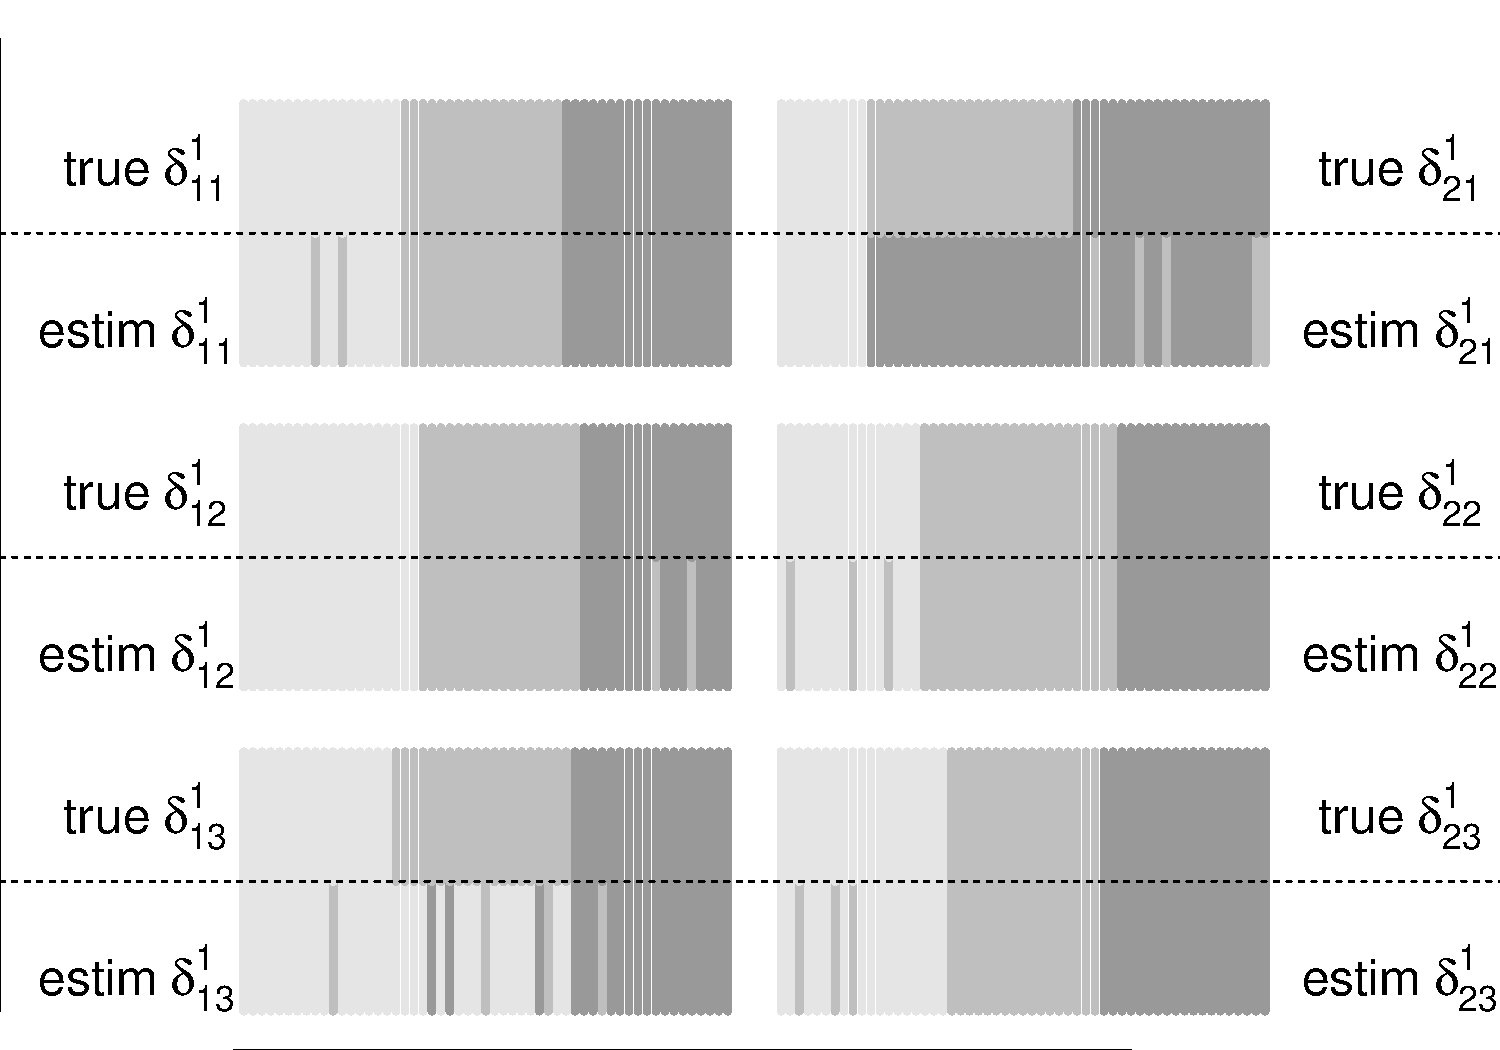
\includegraphics[width=.4\textwidth]{figs_biometrics/cluster_membership_delta1.pdf}
    &
    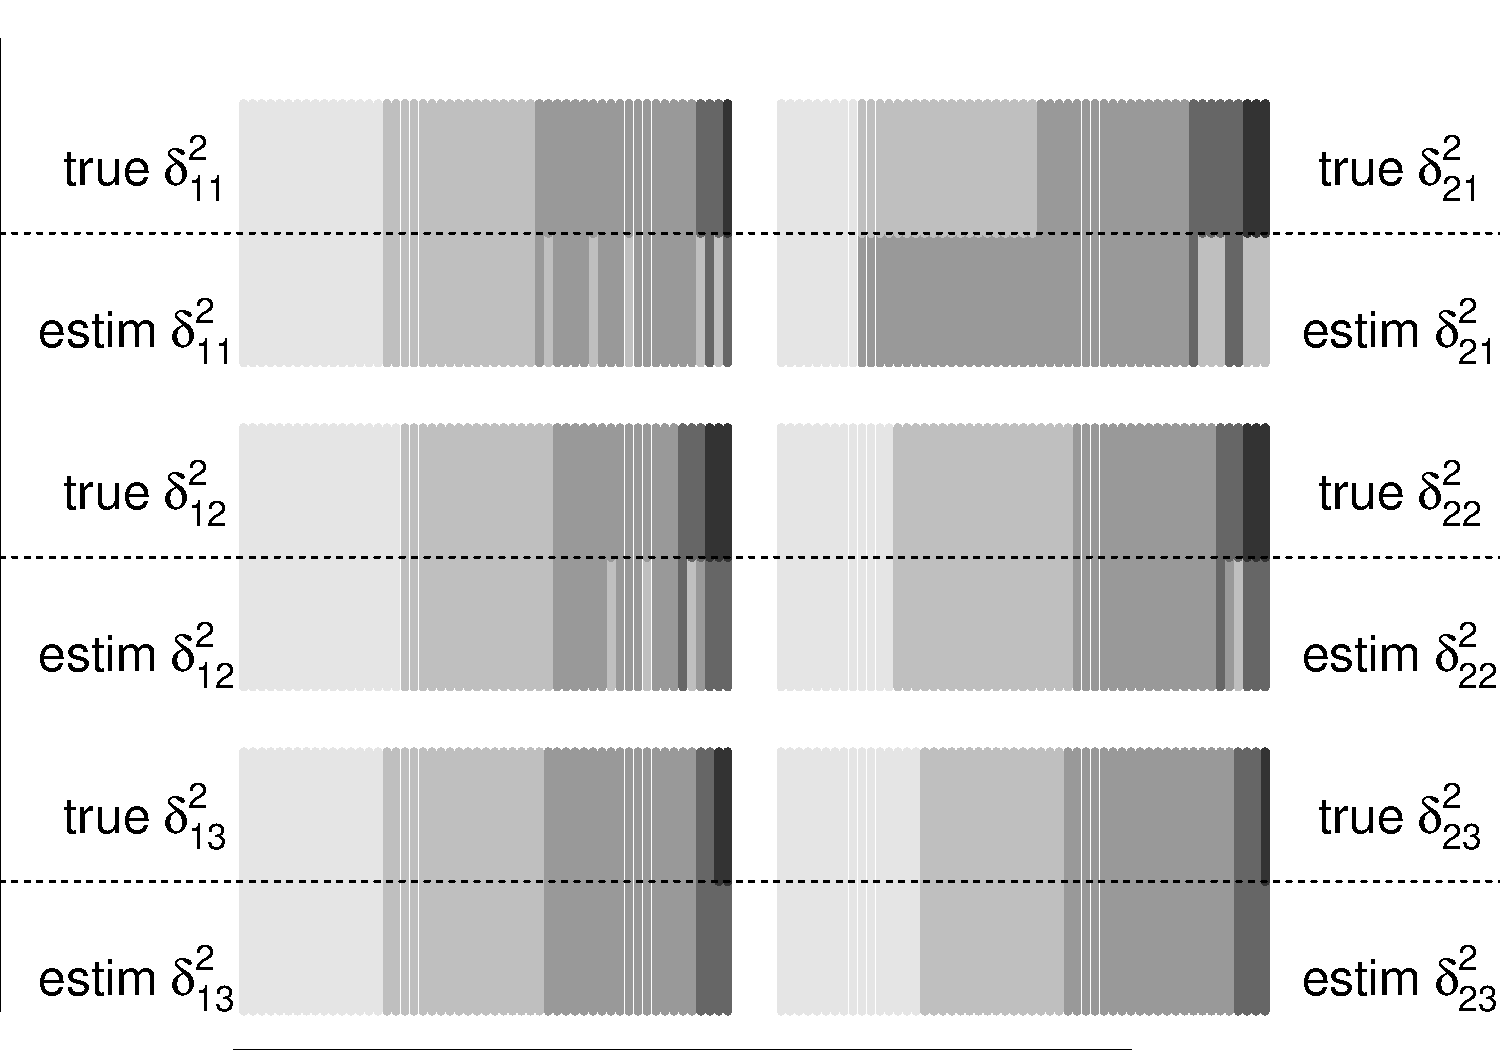
\includegraphics[width=.4\textwidth]{figs_biometrics/cluster_membership_delta2.pdf}\\
    \hspace{0.8 cm} proteins \hspace{0.5cm} proteins &
    proteins \hspace{1cm} proteins \\[4pt]
    (a) Coagulation: $t\leq \tau^1_{cd\ell},$ \ $t > \tau^2_{cd\ell}$& (b) Refinement: \ $\tau^1_{cd\ell} < t \leq \tau^2_{cd\ell}$\\[.5cm]
  \end{tabular}
  % \rotatebox{90}{\hspace{5cm} clusters}\\
  \end{center}
  \caption{Scenario 1:
    Simulation truth $\delta^u_{cd}$ (above horizontal lines) and posterior
    estimated $\deltabar^u_{cd}$ (bellow horizontal lines).
    Each vertical bar corresponds to a gene, with colors (grayscale)
    representing their respective estimated cluster memberships.}
  \label{fig:simulation_cluster_membership}
\end{figure}

Figure \ref{fig:mean_curves_simulation} shows estimated cluster membership and
mean responses (first two columns) in comparison with the
simulation truth (last two columns) for one specific combination of cell
line and drug $(c=2,d=3)$.
Comparing the simulation truth in column 4 with the estimated means in
column 2 we find a good fit for the data.
With one less cluster in the refinement stage picked by BIC, the model merges the two new clusters (darkest shades of gray in columns 3 and 4) into only one
(darkest shade of gray in columns 1 and 2), still providing a good fit with a more parsimonious model.


\begin{figure}[tbp]
%\begin{center}
 \hspace{1.5cm} $\ybar_{it}$ by $\hat{\delta}$ \hspace{0.8cm}
  $E(\mu^*_{\ell u}(m) \mid y,\hat{\delta})$     \hspace{.8cm}
  $\ybar_{it}$ by true  $\delta$           \hspace{.81cm} 
  true $\mu^*_{\ell,u}(m)$\\
  \rotatebox{90}{\hspace{.5cm} dose $\ell=3$ \hspace{1.5cm}
                               $\ell=2$ \hspace{1.5cm}
                               $\ell=1$ \hspace{1.5cm}
                               $\ell=0$                             }
  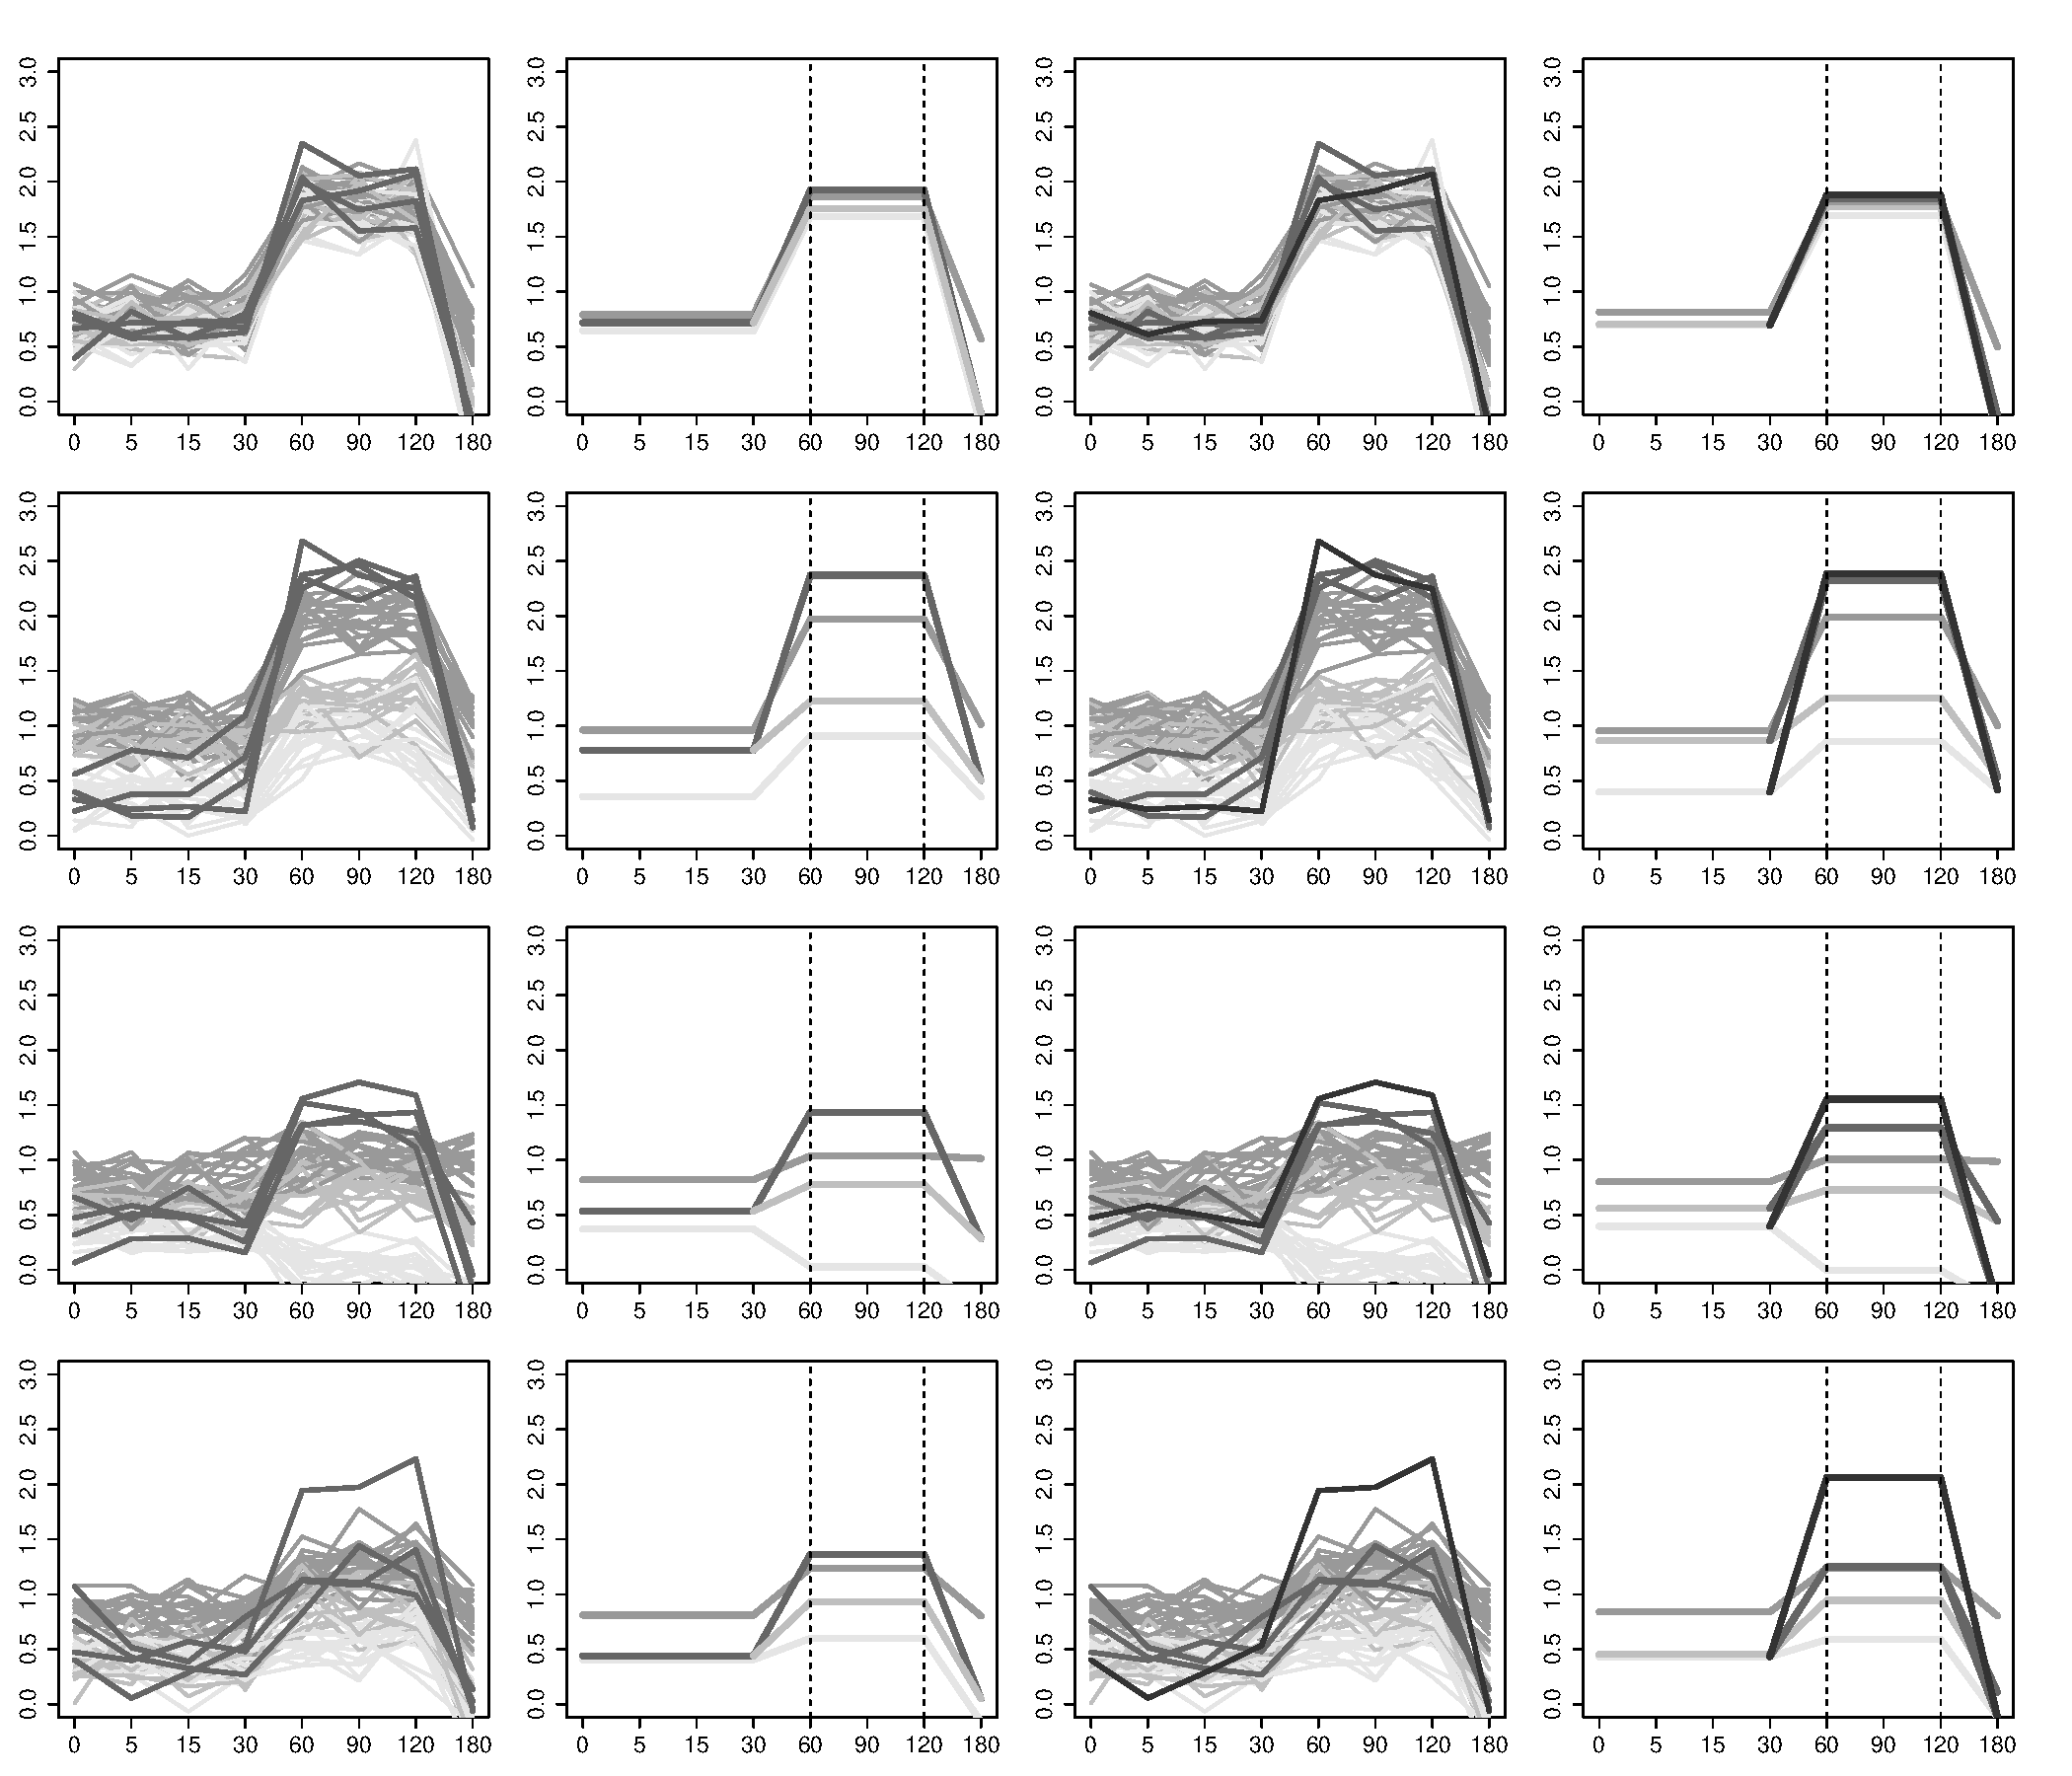
\includegraphics[scale=0.4]{figs_biometrics/sim_35_scenario1_23.pdf} \\
%  \includegraphics[scale=0.4]{figs_biometrics/results_cc_2_d_3_ver3} \\
% \end{center}  
  
\caption{Scenario 1: Mean-response estimation for one of the simulated cases (cell
  line 2, drug 3). Each row corresponds to a different (increasing) dosage level.
  Time is measured in minutes on the horizontal axis.  Column 1 and 3: average over repetitions,
  $\ybar_{it} = \frac{1}{J}\sum^J_{j=1}
  y_{\ell ijt}$ for the 55 proteins. Each line corresponds to a specific
  protein and the color (grayscale) indicates the posterior estimated cluster
  (column 1) and the true cluster (column 3).  Column 2 and 4: posterior
  estimates (column 2) and simulation truth (column 4) for $\mu_{i\ell
    t}$ with dashed lines denoting
  estimated refinement and coagulation times $\tau^1_{\ell}$ and
  $\tau^2_{\ell}$. }
 \label{fig:mean_curves_simulation}
\end{figure}
%\note{Caption: Each row is a different dose (the last row is NOT the average of the previous ones) -- C}

\underline{Scenario 1a. }
We explore prior sensitivity with respect to
the prior on the random partitions and the structure of partitions
over time.
We first repeat inference, still with the same data as in scenario 1; but with a different
hyperprior on the random partition, namely 
$\bfpi_1 \sim \Dir (0.1, \ldots, 0.1)$ and 
$\bfpi_2 \sim \Dir(0.1, \ldots, 0.1)$.
Comparing Figure \ref{fig:sc1ab}(a) with the second column of Figure
\ref{fig:mean_curves_simulation} we find no difference with respect to
the estimated mean responses. 


\begin{figure}[tbp]
  \begin{center}
    %\includegraphics[width=.9\textwidth]{figs_biometrics/sim35_dir_y_23}
  %\rotatebox{90}{\hspace{1.5cm}~  $\ybar_{it}$ by $\hdelta$ }\\
  % \\[4pt]
%    \includegraphics[width=.9\textwidth]{figs_biometrics/sim35_dir_mu_23} %\\[4pt]    
    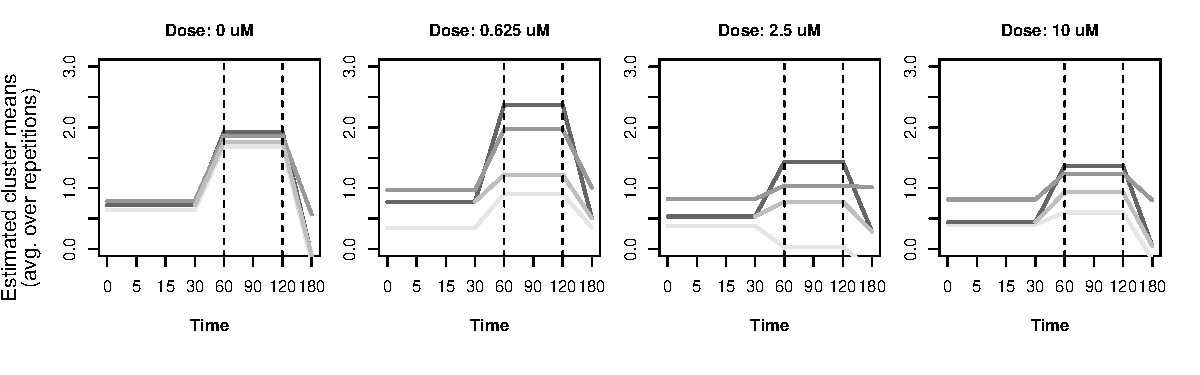
\includegraphics[width=.9\textwidth]{figs_biometrics/sim35_1a_gray_biom23.pdf} %\\[4pt]    
  \rotatebox{90}{\hspace{0.8cm}~$E(\mu^*_{\ell u}(m) \mid y,\hat{\delta})$ }\\
    (a) $\bfpi_1 \sim \Dir(0.1, \ldots, 0.1)$ 
    and $\bfpi_2 \sim \Dir(0.1, \ldots, 0.1)$.\\
    \vspace{1.0cm}
    % (a) $\pi_1 \sim \Dir ( \underbrace{0.1, ..., 0.1}_{\kappa_1})$ \ \ $\pi_2 \sim \Dir(\underbrace{0.1, ..., 0.1}_{\kappa_2 - \kappa_1})$.\\[4pt]
    %\includegraphics[width=.9\textwidth]{figs_biometrics/sim35_gamma_y_23.pdf}
  %\rotatebox{90}{\hspace{1.5cm}~  $\ybar_{it}$ by $\hdelta$ }\\
    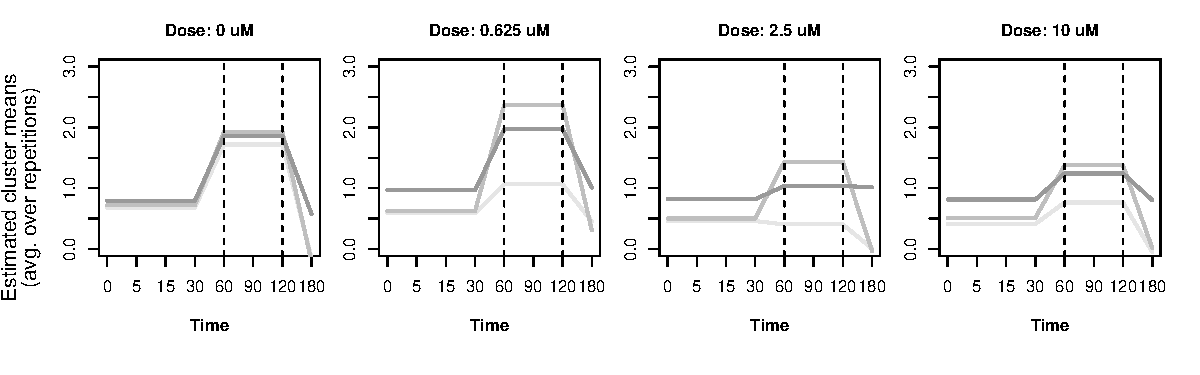
\includegraphics[width=.9\textwidth]{figs_biometrics/sim35_1b_means_23.pdf}
  \rotatebox{90}{\hspace{0.8cm}~$E(\mu^*_{\ell u}(m) \mid y,\hat{\delta})$ }\\
    (b) Single partition model: $\bfdelta^2_{cd}=\bfdelta^1_{cd}$.
  \end{center}

\caption{Scenarios 1a and 1b: Inference under two variations of the prior
  model. Colors (grayscale) denote estimated clusters.
  Panel (a) shows inference under an alternative hyperprior with a
  symmetric Dirichlet prior, 
  $\bfpi_1 \sim \Dir(0.1,\ldots, 0.1)$ and
  $\bfpi_2 \sim \Dir(0.1,\ldots, 0.1)$.
  Panel (b) shows inference 
  using a single invariant partition of proteins over time, i.e.,
  $\bfdelta^2_{cd}=\bfdelta^1_{cd}$.}
\label{fig:sc1ab}
\end{figure}

\underline{Scenario 1b. }
Alternatively we consider inference under a single random partition
that remains invariable over time, that is, using
$\bfdelta^2_{cd}=\bfdelta^1_{cd}$ for all $c$ and $d$, but still allowing changing mean levels over time
as in \eqref{eq:mu_vec}.
Figure \ref{fig:sc1ab} summarizes the resulting inference by showing the
simulated data and the estimated clusters, using the same format as
first and fourth columns in Figure  \ref{fig:mean_curves_simulation}.
Comparing Figure \ref{fig:sc1ab}(b) with the second column of Figure
\ref{fig:mean_curves_simulation} shows a substantially deteriorated
fit under the reduced model without the refined partition.
\smallskip



\underline{Scenario 2:}
We consider another hypothetical scenario with a simulation truth that
closely mimicks the estimated effects in the actual RPPA data
analysis. 
The data $y_{cdi\ell j t}$ are simulated with parameters
fixed at the posterior estimates obtained in section \ref{sec:results}, with $(\kappa_1, \kappa_2)=(4,6)$.
%
Figure \ref{fig:sc2} summarizes simulation results for $c=2$ and $d=1$. 
Using the BIC criterion we select $(\kappa_1,\kappa_2)=(4,6)$,
matching the simulation truth (with $(\kappa_1,\kappa_2)=(4,7)$ and
$(5,6)$ being second and third best). Overall, the cluster-specific means are accurately estimated and
the model fits the simulated data, indicating that inference under
the proposed model can report meaningful summaries for the motivating RPPA data.

\begin{figure}[tbp]
\begin{center}
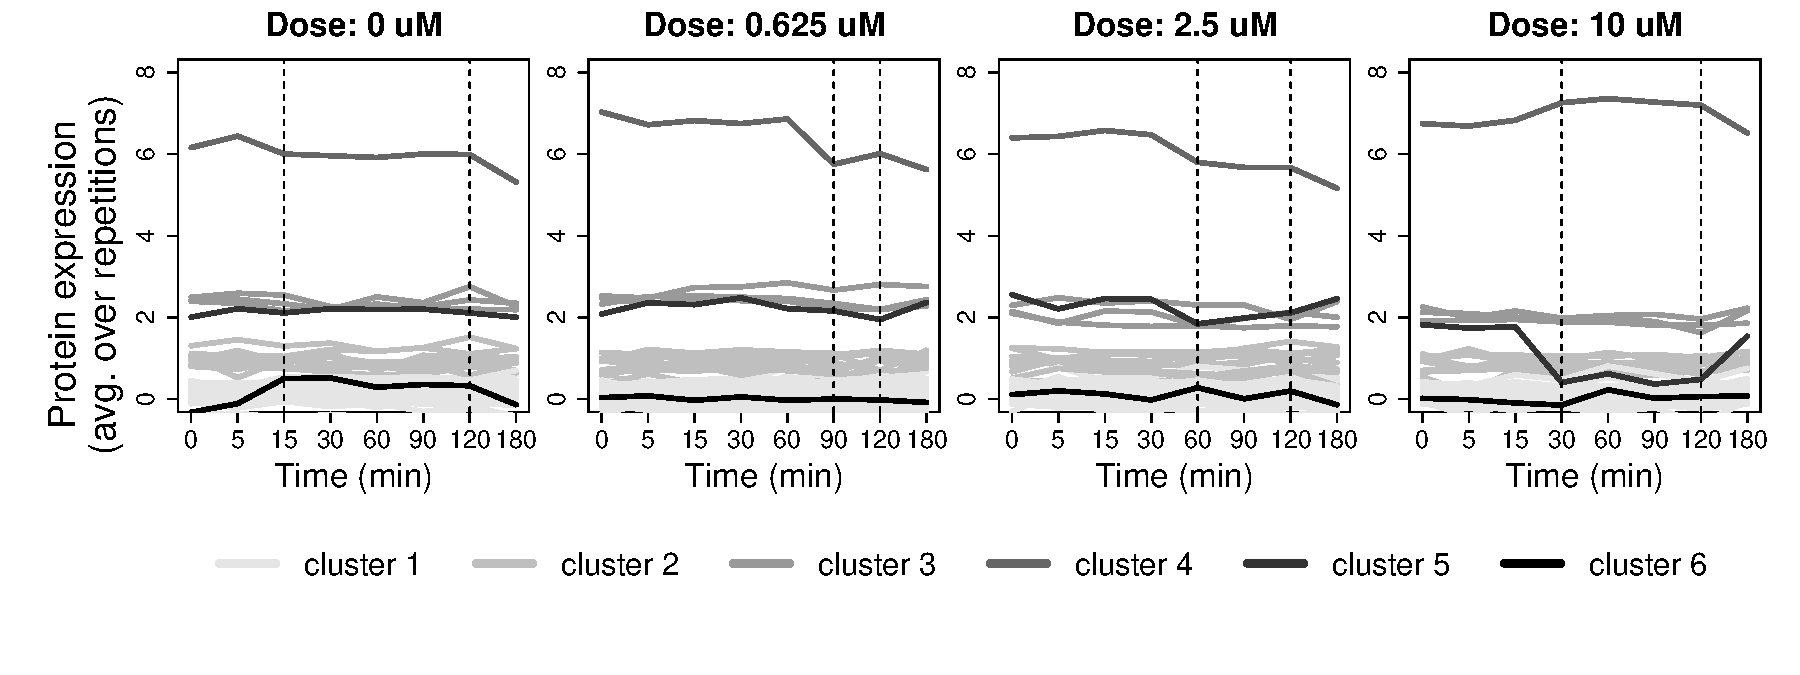
\includegraphics[width=.95\textwidth]{figs_biometrics/scenario2_y_gray_21}\\
(a) Simulated data (over 4 doses). Data for each protein is shown as a
connected line over time. Colors (grayscale) indicate cluster membership
under the simulation truth.\\[4pt]
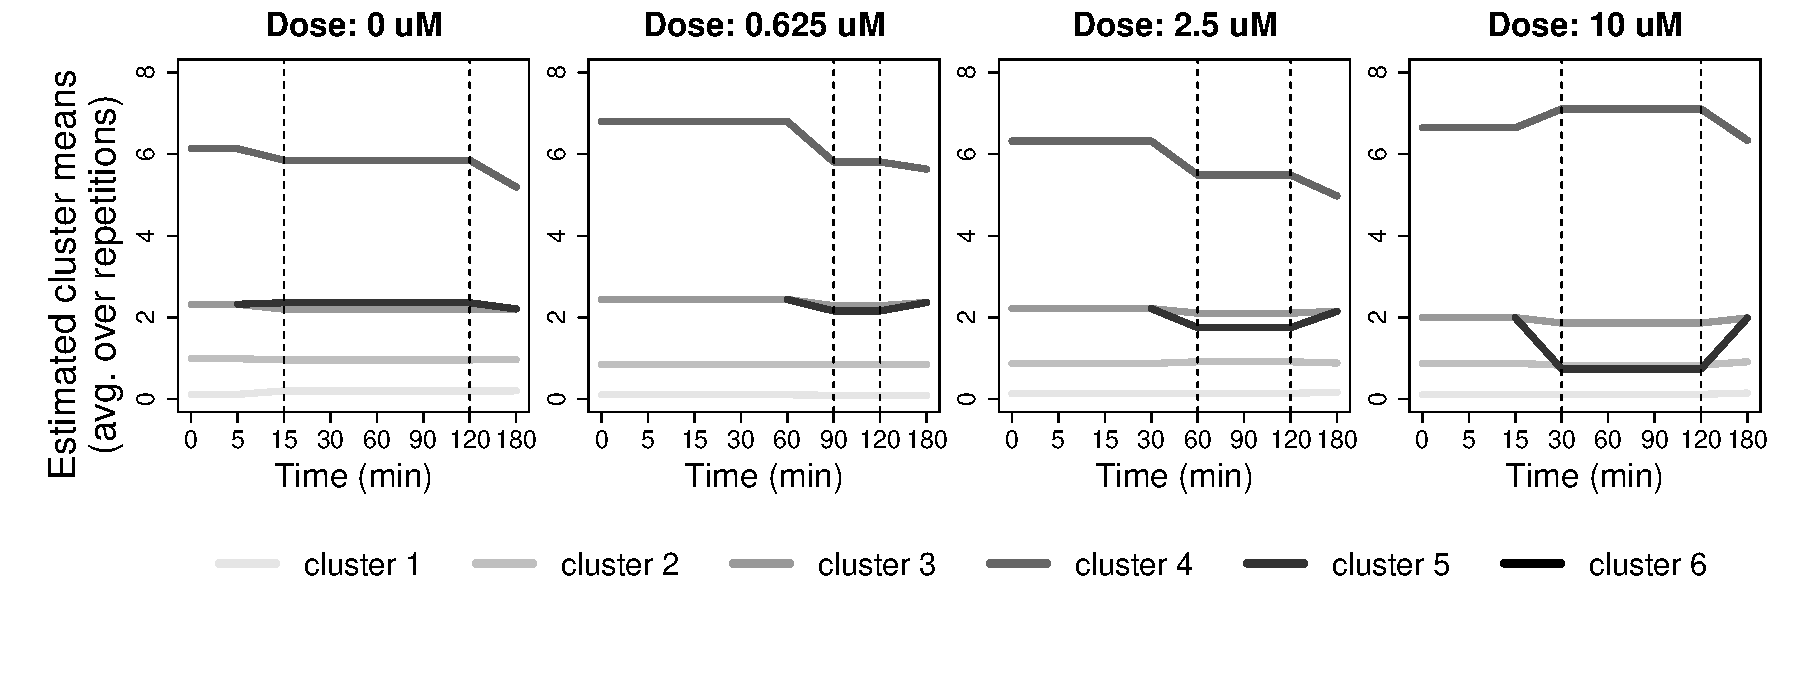
\includegraphics[width=.95\textwidth]{figs_biometrics/scenario2_means_gray_21}\\
(b) Estimated mean expression and cluster memberships. Colors (grayscale) indicate estimated cluster structure.
\end{center}
\caption{Scenario 2. Data (panel a) and estimated mean response and
  cluster membership (panel b).}
\label{fig:sc2}
\end{figure}


\section{Proteomics Data}
\label{sec:results}

Based on BIC we select  $(\kappa_1,\kappa_2)=(4,6)$ (Figure \ref{fig:bic}). While more complex models (with more clusters) exhibit
even better BIC, we find that the results for those models remain very
similar to the ones obtained under $(4,6)$, but with several empty and
redundant clusters. We therefore proceed with the more parsimonious model.

\begin{figure}[tbp]
\centering
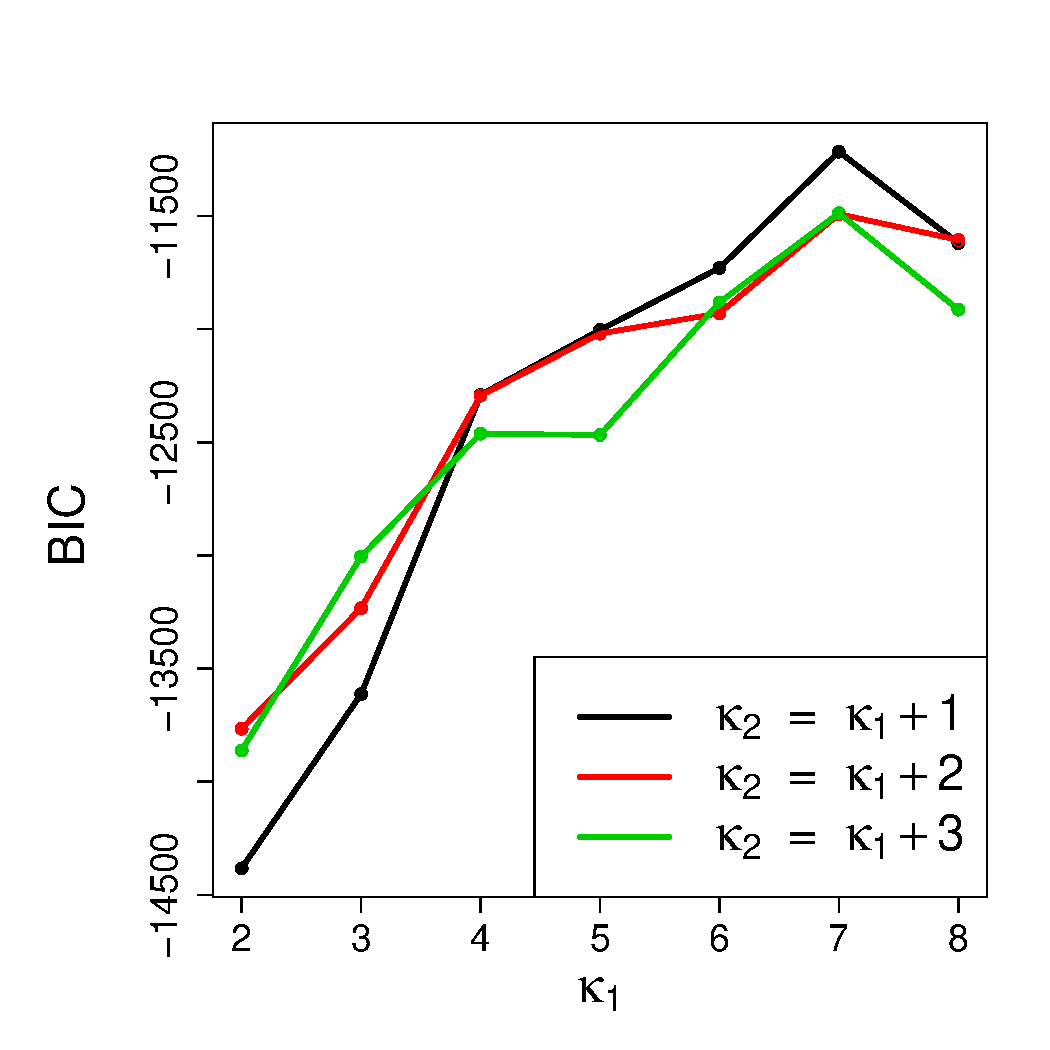
\includegraphics[scale=0.3]{figs_supporting_info/SuppInfo_model_comparison_bic.pdf}
\caption{BIC for different number of clusters $\kappa_1$ and $\kappa_2$ (the bigger, the better).}
\label{fig:bic}
\end{figure}


We implement MCMC simulation for 5,000 iterations discarding the first
2,000 as initial burn-in. Hyperparameters
are fixed as in the simulation study under Scenario 1, i.e.,
$\nu_{\Sigma} = 10$, $\bfV_{\Sigma}=I_{8\times 8}$,
$a_{\gamma}= 1$, $b_{\gamma}= 1$, $\bfeta_1= (1,...,1)^{\top} \in
\mathbb{R}^{\kappa_1}$, $\bfeta_2=(1,...,1)^{\top} \in
\mathbb{R}^{\kappa_2 - \kappa_1}$, $\mu_{00}=0$, $v^{-1}_{00}=0.4444$,
$a_v=1$ and $b_v=1$.



Figures \ref{fig:result_c1_d1} and \ref{fig:result_c2_d1}  show
estimates of the effect of PI3K 
inhibitor on the 55 proteins in cell lines 1 and 2 over time,
respectively.
Cell  line 1 is the cell line MDA-MB-231 and cell line 2 is
MDA-MB-468. Both are derived from a 51-year-old caucasian woman with 
metastatic breast cancer. The two cell lines have been shown to
respond differently to chemotherapies and hormone therapies. Here, the
goal is to characterize response to PI3K inhibition. The following discussion highlights related inference
summaries. Keeping in mind the context of this analysis in the
early phase of a drug development and the moderate sample
sizes, inference should be  understood as hypothesis generating, and
findings should not be over-interpreted.

The first two columns in both figures are as in Figure
\ref{fig:mean_curves_simulation} and show the model fit to the data.
Going from top to bottom (increasing dose) in Figure
\ref{fig:result_c1_d1} one can see that protein
S6 pS235/236
decreases with increased  PI3Ki dose.
At the same time HER2 is activated by the PI3K inhibitor. These two genes
form singletons in our analysis. The inhibition of S6 and activation
of HER2 after PI3K inhibition have been well
reported in the literature
\citep{podsypanina2001inhibitor,serra2011pi3k}. Our analysis for cell
line 1, MDA-MB-231 confirms these findings. In addition, we see
that MAPK pT202Y204 is activated in this cell line as a result of PI3K
inhibition.
We see increased MAPK expression 5 minutes after the PI3K inhibitor is
applied to the samples.
The activation of MAPK as a result of PI3K inhibition is
a major known discovery  in breast cancer~\citep{liu2009targeting}. 

In
contrast, results are different in cell line 2, MAD-MB-468  (Figure
\ref{fig:result_c2_d1}). MAPK is briefly inhibited by
the PI3K inhibitor instead of being activated as in cell line
1. This suggests that cell line 2 includes a mechanism that might reverse the
interactions of PI3K and MAPK. Due to large and complex
down-stream pathways regulated by PI3K, the effects of its inhibition
can be tissue-dependent 
and heterogeneous \citep{engelman2009targeting}. This is shown in the
different response of protein expression in the two cell lines of this
RPPA experiment. The differential response of MAPK to PI3K inhibition
across the two cell lines could be important in interpreting the
reason why they respond differently to therapies.
Discoveries like this are expected to help biologists to set up new hypothesis for further testing.

Summarizing the refinement at time $\tau^1$ as a distance between
$\delta^1$ and $\delta^2$ one could use, for example, the Hamming
distance between co-clustering matrices $P^1$ and $P^2$ with entries
$P^1_{ij}=I(\delta^1_i=\delta^1_j)$ and
$P^2_{ij}=I(\delta^2_i=\delta^2_j)$ respectively.  We find relative
(to the number of pairs) Hamming distances between the partitions
$\delta^1_{cd}$ and $\delta^2_{cd}$ to range from $0.01$ to $0.03$
depending on the cell line $c$ and drug $d$.
% For comparison, the Hamming distance
% evaluated on arbitrary partitions with $I=55$ proteins can assume any
% integer value from 0 to $55\times54/2 = 1485$. 

Table \ref{table_taus} shows point estimates for the refinement and
coagulation times $\tau^1_{\ell }$ and $\tau^2_{\ell }$,
respectively.
For cell line 1 the three drugs (columns) behave similarly,
causing the proteins to refine and revert to te baseline with a similar delay,
% and coagulate at similar time points,
without apparent dose effects. Cell line 2 is different from cell line
1 in that the cells in this line react heterogeneously to the three drugs and
doses. In particular, cell line 1 seems to be more robust to the drugs as the
refinement period is very short across doses. That is, the proteins in
this cell line in general do not react to the drugs. For cell line 2,
proteins seem to be more sensitive to the drugs.  For the first three dose
levels, 0, 0.625, and 2.5 $\mu M$, refinement starts earlier and ends
later with increasing dose levels. This is expected as higher doses
will lead to quick reaction and longer duration of the biological
system. Dose level 10 $\mu M$ is an outlier with a very short
refinement period again. This might be due to the high 
potency of the high drug concentration (10 $\mu M$ is the highest dose level).

\begin{table}[tbp]
\centering \caption{Estimated (mode) refinement and coagulation times
(minutes): $\tau_{\ell }^u$ for cell line $c$, drug $d$, dose $\ell$ and $u
\in \{1, 2\}$.} \label{table_taus}
\resizebox{\columnwidth}{!}{%
\begin{tabular}{c|cccccc|cccccc}
\multicolumn{1}{l |}{}  & \multicolumn{6}{c|}{cell line 1} & \multicolumn{6}{c}{cell line 2} \\ \cline{1-13}
\multicolumn{1}{c|}{drug}  & \multicolumn{2}{c}{PI3Ki} & \multicolumn{2}{c}{AKTi} & \multicolumn{2}{c|}{MEKi} & \multicolumn{2}{c}{PI3Ki} & \multicolumn{2}{c}{AKTi} & \multicolumn{2}{c}{MEKi} \\ \cline{1-13}
\multicolumn{1}{c|}{dose/time}          & \multicolumn{1}{c}{refin.} & \multicolumn{1}{c}{coag.} & \multicolumn{1}{c}{refin.} & \multicolumn{1}{c}{coag.}& \multicolumn{1}{c}{refin.} & \multicolumn{1}{c|}{coag.}& \multicolumn{1}{c}{refin.} & \multicolumn{1}{c}{coag.}& \multicolumn{1}{c}{refin.} & \multicolumn{1}{c}{coag.}& \multicolumn{1}{c}{refin.} & \multicolumn{1}{c}{coag.} \\ \cline{1-13}
\multicolumn{1}{c|}{0 uM}     & 0            & 15           & 0            & 5           & 0            & 15           & 60            & 120           & 60            & 90           & 5            & 120           \\
\multicolumn{1}{c|}{0.625 uM} & 0            & 15           & 0            & 5           & 0            & 5           & 60            & 90           & 5            & 90           & 60            & 120           \\
\multicolumn{1}{c|}{2.5 uM}   & 0            & 30           & 0            & 5           & 0            & 5           & 30            & 120           & 5            & 120           & 15            & 90           \\
\multicolumn{1}{c|}{10 uM}    & 0            & 30           & 5            & 30           & 0            & 5           & 0            & 30           & 90            & 120           & 30            & 60
\end{tabular}%
}
\end{table}

\begin{figure}[tbp]
% \rotatebox{90}{\hspace{4cm} $\ybar_{it}$ (1st column) and $\mu_{i\ell t}$
%   (2nd column)}
%   \hspace{-.2cm}
\phantom{xx} 
\hskip 2cm $\ybar_{it}$ by $\hat{\delta}$  \hspace{0.8cm} $E(\mu^*_{\ell t}(m)\mid y, \hat{\delta})$
  \hspace{0.9cm} coagulation \hspace{0.9cm} refinement\\
  \rotatebox{90}{\hspace{2cm}dose $\ell=3$ \hspace{1.5cm}
                               $\ell=2$ \hspace{2cm}
                               $\ell=1$ \hspace{2cm}
                               $\ell=0$                             }
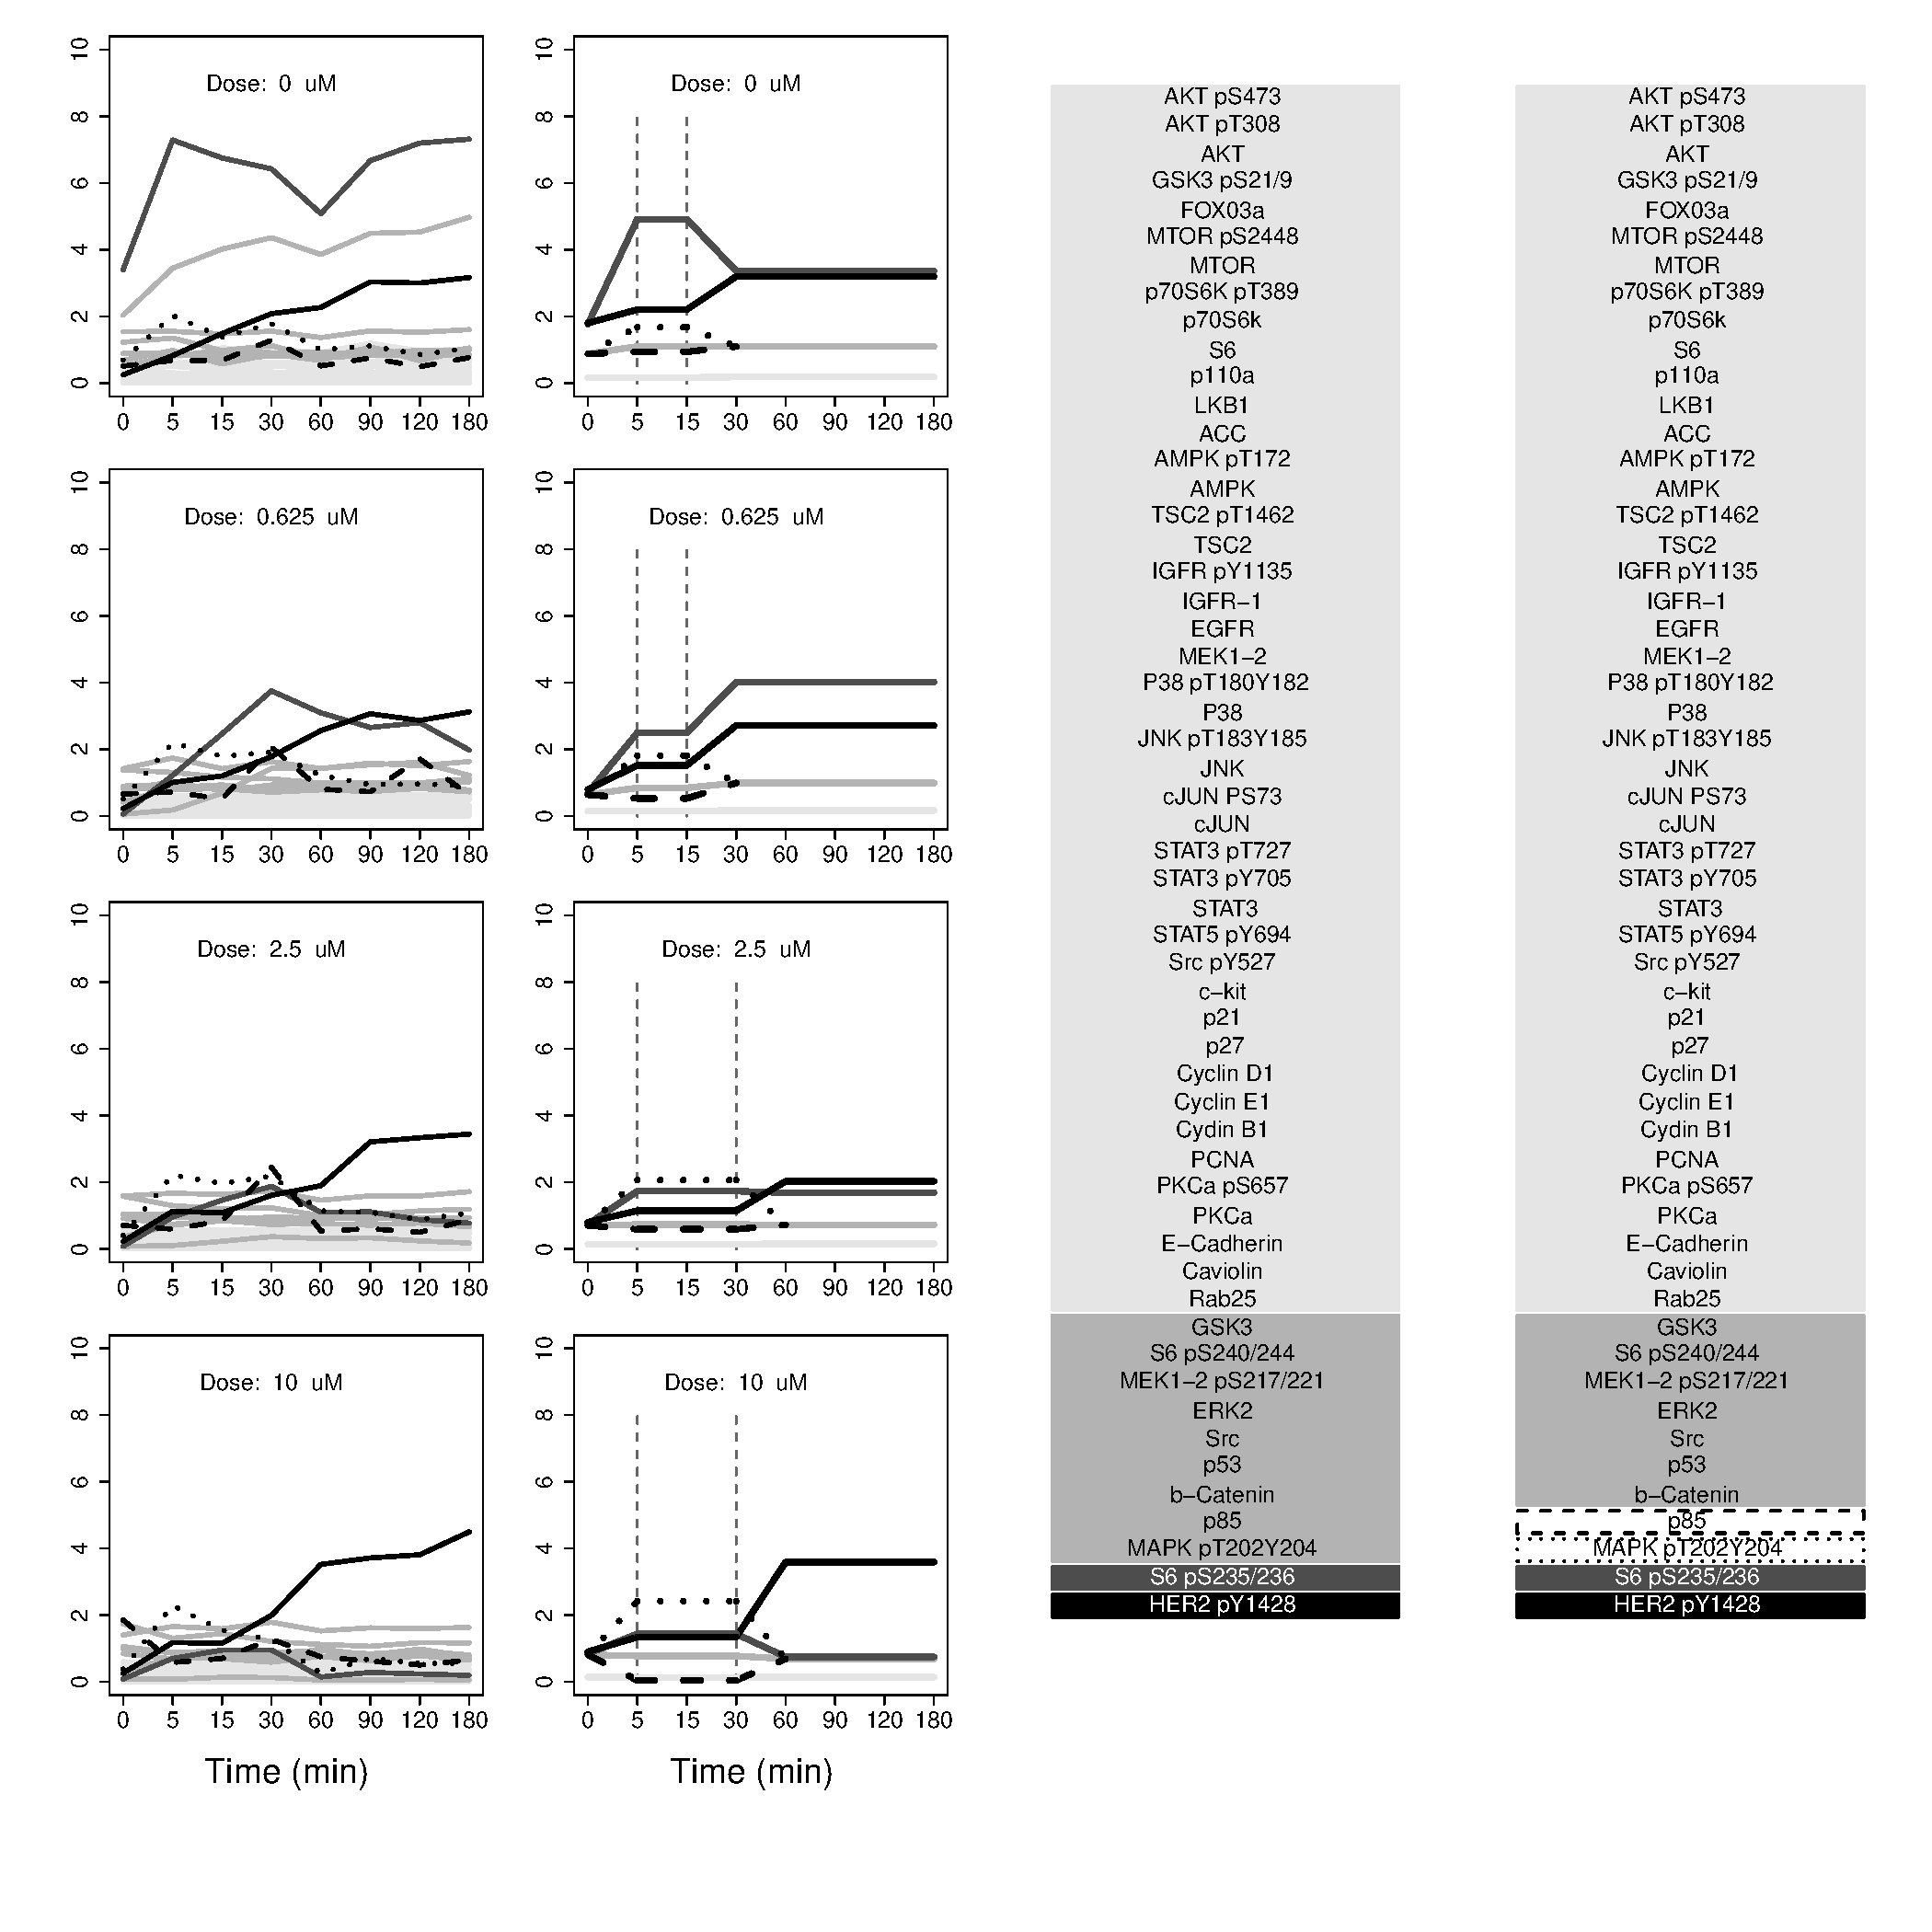
\includegraphics[scale=0.4]{figs_biometrics/results_cc_1_d_1_gray.pdf}\\[-.2cm]
%\phantom{x}{\footnotesize \hspace{1.75cm} TIME}
\caption{Results for proteins in cell line $c=1$ exposed to PI3K inhibitor ($d=1$). Colors (grayscale) denote distinct clusters with dashed lines corresponding to additional clusters formed at refinement.
  Columns 1 and 2 show $\ybar_{it}$ and $\mu_{i\ell t}$ as in
  Figure \ref{fig:mean_curves_simulation}. The horizontal axis contains the observed times
  measured in minutes.
  Columns 3 and 4 show the original partition before refinement
  ($\bfdelta^1_{cd}$, column 3) and
  the refined partition after refinement ($\bfdelta^2_{cd}$, column 4).}
%\note{ {\bf C:} was
 % ``Third
 % column: list of proteins colored by the cluster it belongs to before
 % coagulation and after refinement. Fourth column: same, but with colors
 % corresponding to clusters after coagulation and before refinement.''\\
 % But the 4th column has 2 more clusters, must be the refined partition?}
\label{fig:result_c1_d1}
\end{figure}


\begin{figure}[tbp]
\phantom{xx} 
\hskip 2cm $\ybar_{it}$ by $\hat{\delta}$  \hspace{0.8cm} $E(\mu^*_{\ell t}(m)\mid y, \hat{\delta})$
  \hspace{0.9cm} coagulation \hspace{0.9cm} refinement\\
    \rotatebox{90}{\hspace{2cm} dose $\ell=3$ \hspace{1.5cm}
                               $\ell=2$ \hspace{2cm}
                               $\ell=1$ \hspace{2cm}
                               $\ell=0$                             }
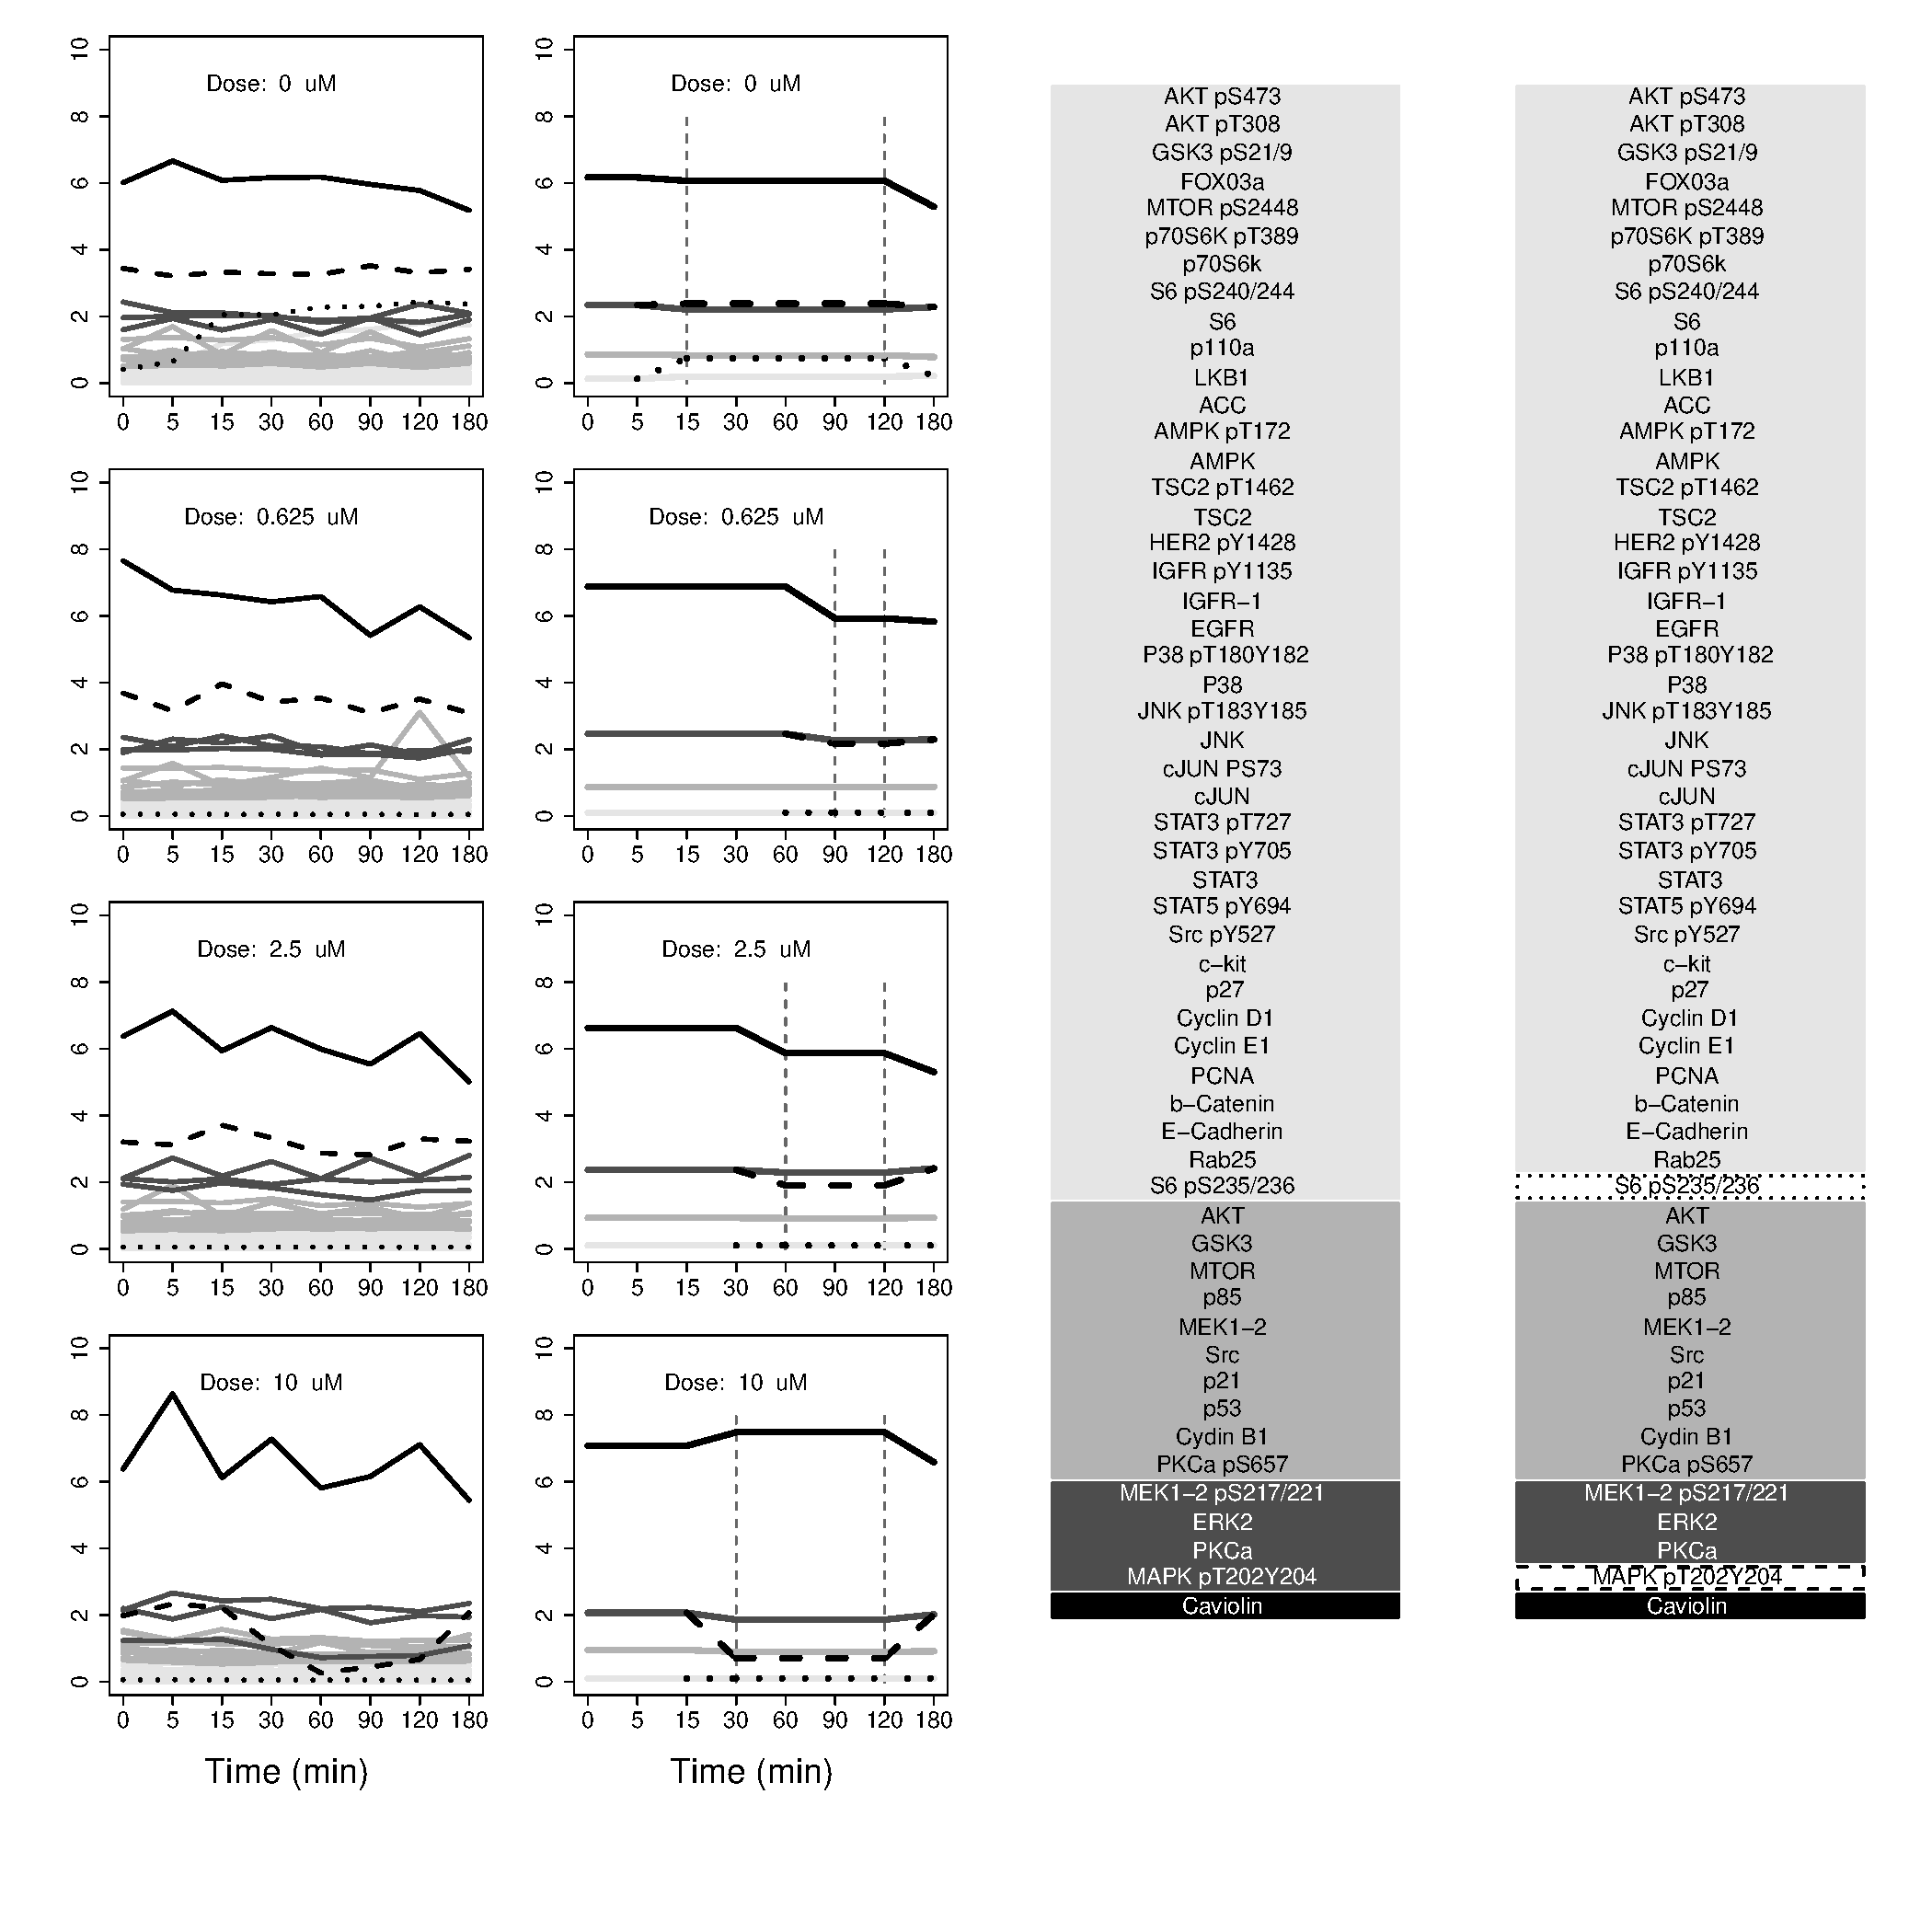
\includegraphics[scale=0.4]{figs_biometrics/results_cc_2_d_1_gray.pdf}\\[-.5cm]
%\phantom{x}{\footnotesize \hspace{1.75cm} TIME}
\caption{
Same as Figure \ref{fig:result_c1_d1}, now for cell line $c=2$.}
\label{fig:result_c2_d1}
\end{figure}


Additionally, in Figure \ref{fig:eda} we illustrate the benefit of the
time-dependent clustering, with only two change points when the
partition changes.
In the figure we explore the use of independent clustering at each
time point, using k-means for an easy implementation.
While one could still identify a small number of proteins that seem
to have their expression gradually increased or decreased at higher
doses of the PI3K inhibitor, there is substantially more noise in the
summary than in the corresponding plot in Figures
\ref{fig:result_c1_d1} and \ref{fig:result_c2_d1}.


\begin{figure}[tbp]
\centering
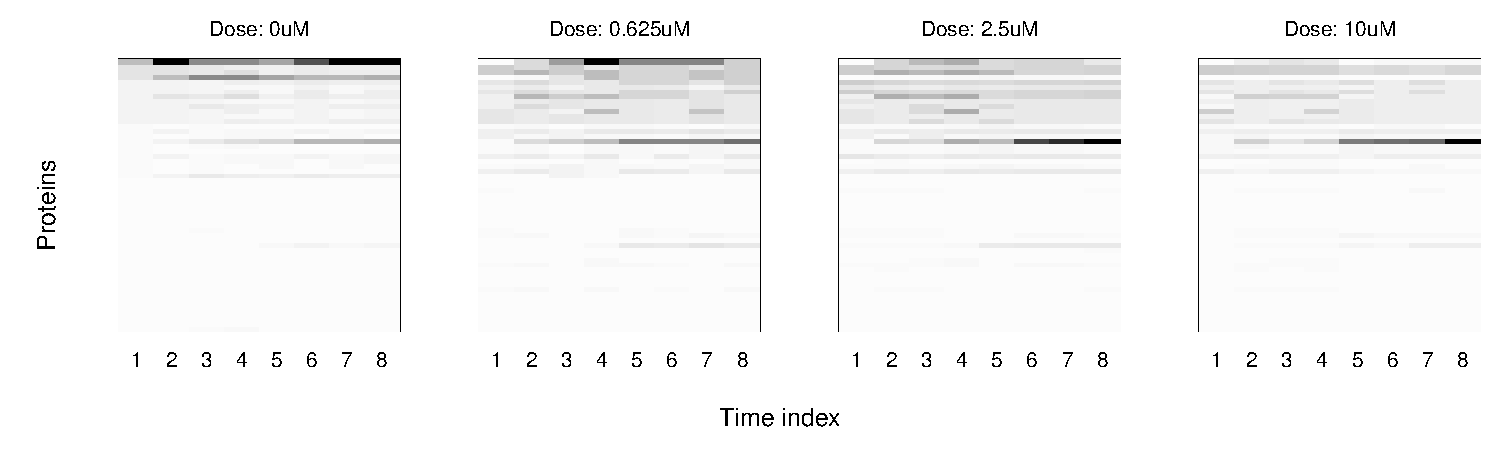
\includegraphics[scale=0.55]{figs_supporting_info/SuppInfo_ea_partition_times_11}
%\includegraphics[scale=0.6]{newfigs/ea_partition_times_11}
\caption{Independent k-means (k=5) estimation of partitions across time for different doses of PI3K inhibitor administered to cell line 1. For a fixed column (time index), each color represents the estimated cluster specific mean for that particular protein (higher expressions are darker).}
\label{fig:eda}
\end{figure}


% shows a preliminary estimation of the partitions
% carried out by k-means indepently across time. This approach is not
% capable of sharing information across time and as a result the cluster
% configurations exhibit wide variation for consecutive times that is
% likely to be simply random noise. 

\section{Discussion}
We introduced a model for finding a subpopulation of proteins that are
most affected by a particular intervention. The key element of the
model is a sequence of random partitions subject to the desired
monotonicity. The same inference -- without any change in the
probability model -- can be interpreted as inference on
% a change point in
mean protein expression over time, with the clusters serving
the purpose of adaptively borrowing strength across proteins, doses,
drugs and cell lines. The latter happens only at the level of
hyperparameters.  The approach is meaningful in any inference problem
with a sequence of partitions that include a notion of
monotonicity. It is most appropriate when limited data or high
noise leaves more complexly structured models impractical to fit.

Several extensions and generalizations of the proposed model are
possible. With more data one could replace the piecewise constant
mean response by a piecewise linear mean response with little change
in the remaining model. In the application to the RPPA data it was
reasonable to assume that once the treatment effect wears off the mean
response would revert to the initial levels. Other applications might
call for lasting treatment effects, allowing for a different final
level. Also, in other applications the use of more than two change
points might be meaningful, with possibly different sequences of
refinements and coagulations.

In the discussion following equation \eqref{eq:lik} we commented on alternative priors on $\Sigma_c$. In an application with richer data one could alternatively consider a Gaussian Process prior with more general covariance structure.

The main limitation is the computationally awkward problem of estimating
the size of the partitions. With respect to the application, a limitation
is that the described inference targets only mean expression levels,
missing changes that are in the dependence structure. The latter is
plausible when the intervention affects pathways and feedback mechanisms.
